\chapter{Graph Neural Network Flavour Tagger}\label{chap:gnn_tagger}

As discussed in \cref{chap:tracking}, flavour tagging is the identification of jets instantiated from \bchadrons.
Flavour tagging is a critical component of the physics programme of the ATLAS experiment. 
It is of crucial importance for the study of the Standard Model (SM) Higgs boson and the top quark, which decay preferentially to \bquarks \cite{HIGG-2018-04,HIGG-2018-13}, and additionally for several Beyond the Standard Model (BSM) resonances that readily decay to heavy flavour quarks \cite{EXOT-2019-03}.

This chapter introduces \GNN, a novel ML-based flavour tagging algorithm based on graph neural networks (GNNs).
In \cref{sec:gnn_motvation}, an overview of the approach used for \GNN is provided.
An introduction to the theory of GNNs is provided in \cref{sec:gnn_theory}.
Details of the experimental setup are provided in \cref{sec:experimental_setup}, while the architecture of \GNN is specified in \cref{sec:Architecture}.
In \cref{sec:training}, the training procedure is described, and in \cref{sec:gnn_results} the results are shown.

\section{Motivation}\label{sec:gnn_motvation}

\GNN is a monolithic approach to flavour tagging as illustrated in~\cref{fig:oldvsnew}.
As opposed to the existing approach to flavour tagging described in \cref{chap:tracking}, which relies on a two tiered approach requiring the use of both low- and high-level algorithms,
\GNN takes as inputs information directly from an unordered variable number of tracks as input, and predicts the jet flavour without requiring outputs from the intermediate low-level algorithms.
In addition to predicting the flavour of the jet, the model predicts which physical processes produced the various tracks, and groups the tracks into vertices.
These auxiliary training objectives provide valuable additional information about the contents of the jet and enhance the performance of the primary flavour prediction task.
The use of GNNs offers a natural way to classify jets with variable numbers of unordered associated tracks (see \cref{sec:gnn_theory}), while allowing for the inclusion of auxiliary training objectives~\cite{2020-gnn-for-sv,serviansky2020set2graph}.

\begin{figure}[!htbp]
    \centering
    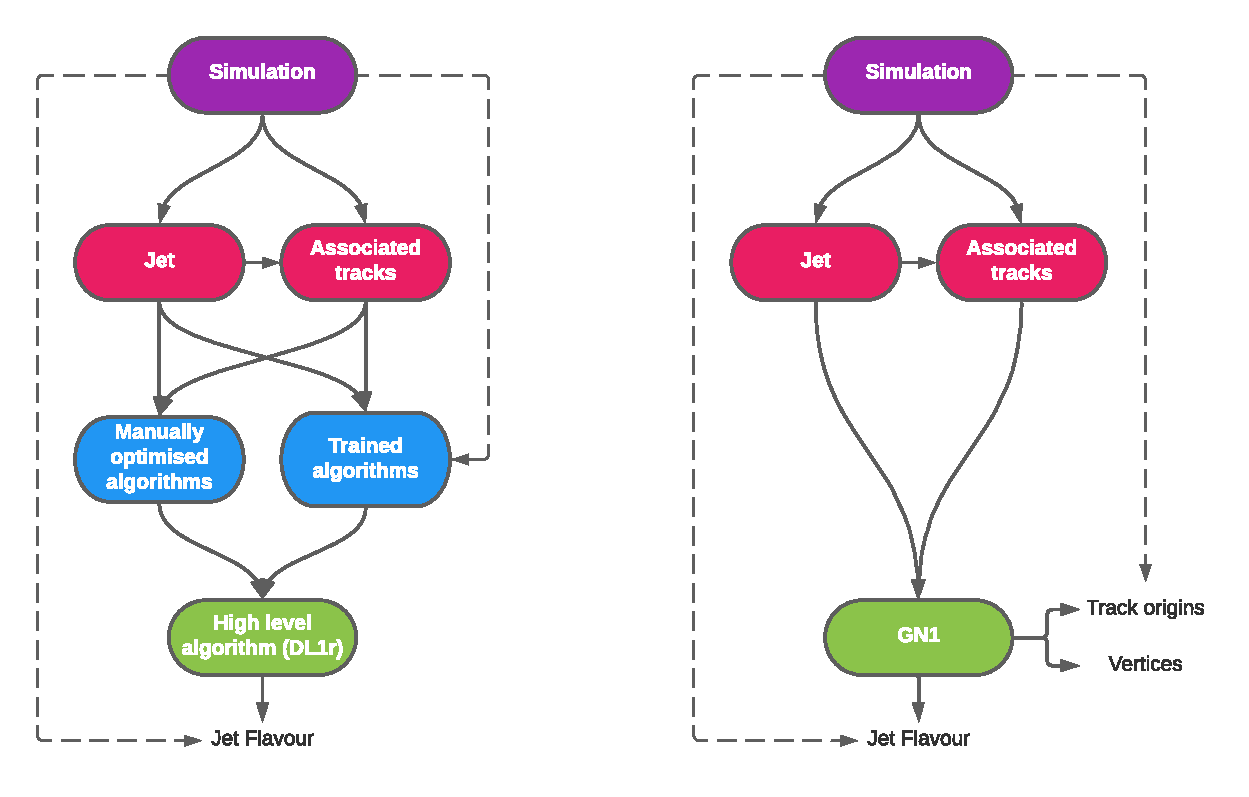
\includegraphics[width=0.9\textwidth]{chapters/gnn_tagger/figs/GNN_compare_contrast.pdf}
    \caption{Comparison of the existing flavour tagging scheme (left) and \GNN (right) \cite{ATL-PHYS-PUB-2022-027}. The existing approach utilises low-level algorithms (shown in blue), the outputs of which are fed into a high-level algorithm (\DLr). Instead of being used to guide the design of the manually optimised algorithms, additional truth information from the simulation is now being used as auxiliary training targets for \GNN. The solid lines represent reconstructed information, whereas the dashed lines represent truth information.}
    \label{fig:oldvsnew}
\end{figure}

As described in \cref{chap:tracking}, current flavour tagging algorithms utilise a two-tired approach.
The high-level tagger \DLr outputs variables which provides good discrimination between the different jet flavours.
In contrast \GNN consists of only a single neural network, which the tracks as inputs along with some kinematic information about the jet.
As a result, it does not depend on the outputs of any other flavour tagging algorithm.
A simple training of the model fully optimises its parameters, represting a significant simplification with respect to the optimisation procedure for \DLr.
This is particularly important when optimising the tagger for new regions of phase space (e.g. \ctag or \highpt \btag), or when the detector is upgraded or the charged particle reconstruction or selection algorithms are re-optimised.

\GNN is trained to learn about the internal structure of the jet through the use of two auxiliary training objectives: the prediction of the underlying physics process from which each track originated, and the grouping of tracks originating from a common spatial position (i.e. a common vertex).
These auxiliary objectives are meant to guide the neural network towards a more complete understanding of the underlying physics inside the jet, thereby removing the need for the low-level algorithms, which previously contained information about the underlying physics in their design.
The training targets for the primary and auxiliary objectives are extracted from truth information, i.e. information that is only available in simulation, as opposed to reconstructed quantities available in both collision data and simulation.

In this chapter, the following advantages of the \GNN approach will be demonstrated:

\newcommand{\fakesfootnote}{%
A fake track is defined as a track with a truth-matching probability less than $0.5$, where the truth-matching probability is defined in Ref.~\cite{PERF-2015-08}.
}
\begin{enumerate}
    \item \GNN boasts improved performance with respect to the current ATLAS flavour tagging algorithms, with significantly larger background rejection rates for a given signal efficiency. Alternatively the rejection rates can be kept fixed for a substantial increase in signal efficiency, in particular at \highpt.
    \item The same network architecture can be easily optimised for a wider variety of use cases (e.g. \cjet tagging and \highpt jet tagging) since there are no low-level algorithms to retune.
    \item There are fewer algorithms to maintain.
    \item Alongside the network's prediction of the jet flavour, the auxiliary vertex and track origin predictions provide more information on why a jet was (mis)tagged or not. This information can also have uses in other applications, for instance to explicitly reconstruct displaced decay vertices or to remove fake tracks.\footnote{\fakesfootnote}
\end{enumerate}



\section{Experiemental Setup}\label{sec:experimental_setup}

\subsection{Datasets}\label{sec:datasets}

The datasets used to train the \GNN tagger are the same as described in \cref{sec:track_classifier_datasets}.
The training dataset contains \njetstrain jets, \pct{60} of which are \ttbar jets and \pct{40} of which are \Zprime jets.
%Although \DLr uses \pct{70} \ttbar jets and \pct{30} \Zprime jets, the composition of the training samples was found to have a negligible impact on the final performance of \GNN.
In order to evaluate the performance of the model during, a statistically independent set of \njetsval testing jets from both the \ttbar and \Zprime samples are used.
For the final testing of the model and the creation of the performance plots, a further 1 million independent testing jets from each of the \ttbar and \Zprime samples are used.
Before being fed into the model, the track- and jet-level inputs are normalised to have a mean of zero and a variance of unity. 
The jet flavour labels are assigned as described in \cref{sec:jet_reco}.
Truth labelled \bcl jets are kinematically re-sampled in \pt and $\eta$ to ensure identical distributions in these variables.


\section{Model Architecture}\label{sec:networks}

\subsection{Model Inputs}\label{sec:model-inputs}

\newcommand{\ipdefsfootnote}{%
Impact parameter significances are defined as the IP divided by its corresponding uncertainty, $\dzerosig = d_0 / \dzerouncert$ and $\zzerosig = z_0 / \zzerouncert$.
Track IP significances are lifetime signed according to the track's direction with respect to the jet axis and the primary vertex \cite{PERF-2012-04}.
}

As inputs, \GNN is fed two kinematic jet variables and an unordered set of up to 40 tracks which have been associated to the jet.
Each track consists of 21 variables.
The kinematic jet variables are the jet transverse momentum and signed pseudorapidity.
The input variables which are provided for each track are listed in \cref{tab:track_inputs}.
%The track parameters and associated uncertainties, along with detailed hit information, are used as these variables carry critical information about the jet flavour.
For each track, variables containing the track parameters and uncertainties, and detailed information on the hit content are provided as inputs to the model.

In cores of \highpt jets, track density is high due to the increased multiplicity and collimation of tracks (see \cref{chap:tracking}).
As a result, the separation between tracks can be of the same order as the active sensor dimensions, resulting in an increase in merged clusters and tracks which share hits \cite{PERF-2015-08}.
Due to the relatively long lifetimes of \bhadrons and \chadrons, which can traverse several layers of the ID before decaying and have highly collimated decay products, the presence of shared or missing hits is a critical signature of heavy flavour jets.

Dependence of the model on the absolute value of the azimuthal jet angle $\phi$ is explicitly removed by providing only the azimuthal angle of tracks relative to the jet axis. The track pseudorapidity is also provided relative to the jet axis.
%The sign of the jet pseudorapidity is included, but could be removed in the future to also build in the forward-backwards symmetry present at ATLAS.

Since heavy flavour hadrons can decay semileptonically approximately \pct{20} of the time, the presence of a reconstructed lepton in the jet carries discriminating information about the jet flavour. 
% (note this is 20% directly for b-hadrons and 20% for c-hadrons, so 40% overall)
To exploit this, a variant of \GNN called \GNNLep is trained in addition to the baseline model.
The \GNNLep variant is identical to the baseline model, except for the inclusion an additional track-level input, leptonID, which indicates if the track was used in the reconstruction of an electron, a muon or neither. 
The variable is signed by the charge of the reconstructed lepton.
The leptons used in the definition of the leptonID variable are required to satisfy basic quality requirements.
The muons are required to be combined \cite{ATL-PHYS-PUB-2015-037}, and the electrons are required to pass the \textit{VeryLoose} likelihood-based identification working point \cite{PERF-2017-01}.

\begin{table}[!htbp]
  \footnotesize\centering
  \setlength{\tabcolsep}{0.5em} % for the horizontal padding
  \begin{tabular}{ll}
    \toprule\hline 
    \textbf{Jet Input} & \textbf{Description} \\
    \hline
    $\pt$ & Jet transverse momentum \\
    $\eta$ & Signed jet pseudorapidity \\
    \toprule
    \textbf{Track Input} & \textbf{Description} \\
    \hline
    $q/p$ & Track charge divided by momentum \\
    $\mathrm{d}\eta$ & Pseudorapidity of the track, relative to the jet $\eta$ \\
    $\mathrm{d}\phi$  & Azimuthal angle of the track, relative to the jet $\phi$ \\
    $\dzero$  & Closest distance from the track to the PV in the longitudinal plane \\
    $\zzero\sin\theta$  & Closest distance from the track to the PV in the transverse plane \\
    $\sigma(q/p)$ & Uncertainty on $q/p$ \\
    $\sigma(\theta)$ & Uncertainty on track polar angle $\theta$ \\
    $\sigma(\phi)$  & Uncertainty on track azimuthal angle $\phi$ \\
    $\dzerosig$  & Lifetime signed transverse IP significance \\
    $\zzerosig$  & Lifetime signed longitudinal IP significance \\
    nPixHits   & Number of pixel hits \\
    nSCTHits   & Number of SCT hits \\
    nIBLHits   & Number of IBL hits \\
    nBLHits    & Number of B-layer hits \\
    nIBLShared & Number of shared IBL hits \\
    nIBLSplit  & Number of split IBL hits \\
    nPixShared & Number of shared pixel hits \\
    nPixSplit  & Number of split pixel hits \\
    nSCTShared & Number of shared SCT hits \\
    nPixHoles  & Number of pixel holes \\
    nSCTHoles  & Number of SCT holes \\
    leptonID   & Indicates if track was used to reconstruct an electron or muon \\
    \hline\bottomrule
  \end{tabular}
  \caption{
    Input features to the \GNN model \cite{ATL-PHYS-PUB-2022-027}.
    Basic jet kinematics, along with information about the reconstructed track parameters and constituent hits are used.
    Shared hits, are hits used on multiple tracks which have not been classified as split by the cluster-splitting neural networks~\cite{PERF-2015-08}, while split hits are hits used on multiple tracks which have been identified as merged.
    A hole is a missing hit, where one is expected, on a layer between two other hits on a track.
    The track leptonID is an additional input to the \GNNLep model.
  }
  \label{tab:track_inputs}
\end{table}

The selections applied to the tracks is the same as that used for the fake track classification MVA described in \cref{chap:track_classification_mva}.
The full set of track selections is listed in \cref{tab:fake_track_mva_selections}.
This selection was found to improve the flavour tagging performance compared to previous tighter selections, whilst ensuring good resolution of tracks and a low fake rate~\cite{PERF-2015-08}.
However, \cref{sec:looser_track_selection} demonstrates that further relaxation of the track selection requirements may be warranted. 

If more than 40 tracks are associated to a given jet, only the first 40 tracks with the largest transverse IP significance\footnote{\ipdefsfootnote} \dzerosig are fed into the model as inputs.

\subsection{Auxiliary Training Objectives}\label{sec:aux-train-objectives}

In addition to the jet flavour classification, two auxiliary training objectives are defined.
The first auxiliary objective is the prediction of the physical process that gave rise to each track within the jet (i.e. the track origin), while the second is the prediction of track-pair vertex compatibility. 
Each auxiliary training objective comes with a training target which, similar to the jet flavour label, is a truth labels derived from the simulation.
The presence of the auxiliary training objectives improves the jet classification performance as demonstrated in \cref{sec:gnn_ablations}.

For the track origin prediction objective, each track is labelled with one of the exclusive categories defined in \cref{tab:truth_origins} of \cref{sec:track_labelling} after analysing the particle interaction (or lack thereof) which led to its formation. 
Since the presence of different track origins is strongly related to the flavour of the jet, training \GNN to recognise the origin of the tracks provides an additional handle on the classification of the jet flavour.
This task may also aid the jet flavour prediction by acting as a form of supervised attention~\cite{arxiv.2007.08294}~-~in detecting tracks from heavy flavour decays the model may learn to pay more attention to these tracks.

The vertexing auxiliary objective makes use of the fact that displaced decays of \bchadrons lead to secondary and tertiary vertices inside the jet, as described in \cref{sec:b_decay_topology}.
The presence of displaced secondary vertices is not a completely clean signal of a heavy flavour jet, as displaced secondary vertices can also occur in \ljets as a result of material interactions, conversions, and long-lived particle decays (e.g. \Kshort and $\Lambda^0$).
For the auxiliary object, \GNN predicts a binary label for each pair of tracks in the jet.
The label has a value of 1 if the truth particles associated with the two tracks in the pair originated from the same spatial point, and 0 otherwise. 
To derive the corresponding truth labels for training, truth production vertices within $0.1$ mm are merged.%, as these are assumed to be unresolvable given the granularity of the ID. 
Track-pairs where one or both of the tracks in the pair have an origin label of either Pileup or Fake are given a label of 0.
Using the pairwise predictions from the model, groups of tracks that have common compatability can be formed, resulting in the finding of vertices.
Two existing low-level tagging algorithms, SV1 and JetFitter (introduced in \cref{sec:vertex_reco}), are currently used to find and reconstruct vertices inside jets and are used as inputs to the existing jet flavour tagger \DLr.
The addition of this auxiliary training objective removes the need for inputs from a dedicated secondary vertexing algorithm.

Both of the auxiliary training objectives described here can be considered as ``stepping stones'' on the way to classifying the flavour of the jet. 
By requiring the model to predict the truth origin of each track and the vertex compatibility of each track-pair, the model is guided to learn representations of the jet which are connected to the underlying physics and therefore relevant for classifying the jet flavour. 


\subsection{Architecture}\label{sec:Architecture}

As discussed in the previous sections, \GNN is a graph neural network which makes use of auxiliary training objectives in order to determine the jet flavour.
A coarse optimisation of the network architecture hyperparameters (for example number of layers and number of neurons per layer) has been carried out in order to maximise the flavour tagging performance, but it is likely that further dedicated optimisation studies could lead to further performance improvements. 

The model architecture builds on a previous implementation of a GNN-based jet tagger~\cite{serviansky2020set2graph}.
The previous approach was comprised of two separate graph neural networks with the auxiliary tasks being performed at an intermediate stage after the first and before the second.
This two stage approach was found to be unnecessary and as such \GNN simplifies the architecture into a single graph neural network with the auxiliary tasks being performed at the end, alongside the primary jet classification task.
\GNN makes use of a more sophisticated graph neural network layer \cite{2021arXiv210514491B}, which is described in more detail below.
The changes significantly improved tagging performance and also led to a significant reduction in training time.

As inputs, the model takes information about the jet and a number of associated tracks, as detailed in \cref{sec:model-inputs}.
The jet variables are concatenated with the variables for each track as shown in \cref{fig:model_input_array}.
The combined jet-track input vectors are then fed into a per-track initialisation network with three hidden layers, each containing 64 neurons, and an output layer with a size of 64, as shown in \cref{fig:new_arch}. 
The track initialisation network is similar to a deep sets model \cite{zaheer2018deep}, but does not include a reduction operation (mean or summation) over the output track representations.
The initialisation network allows for initial per-track input processing without the associated parameter count cost of the graph convolutional layers described below. 
%Additionally, other input types with different input sizes can be 

\begin{figure}[!htbp]
    \centering
    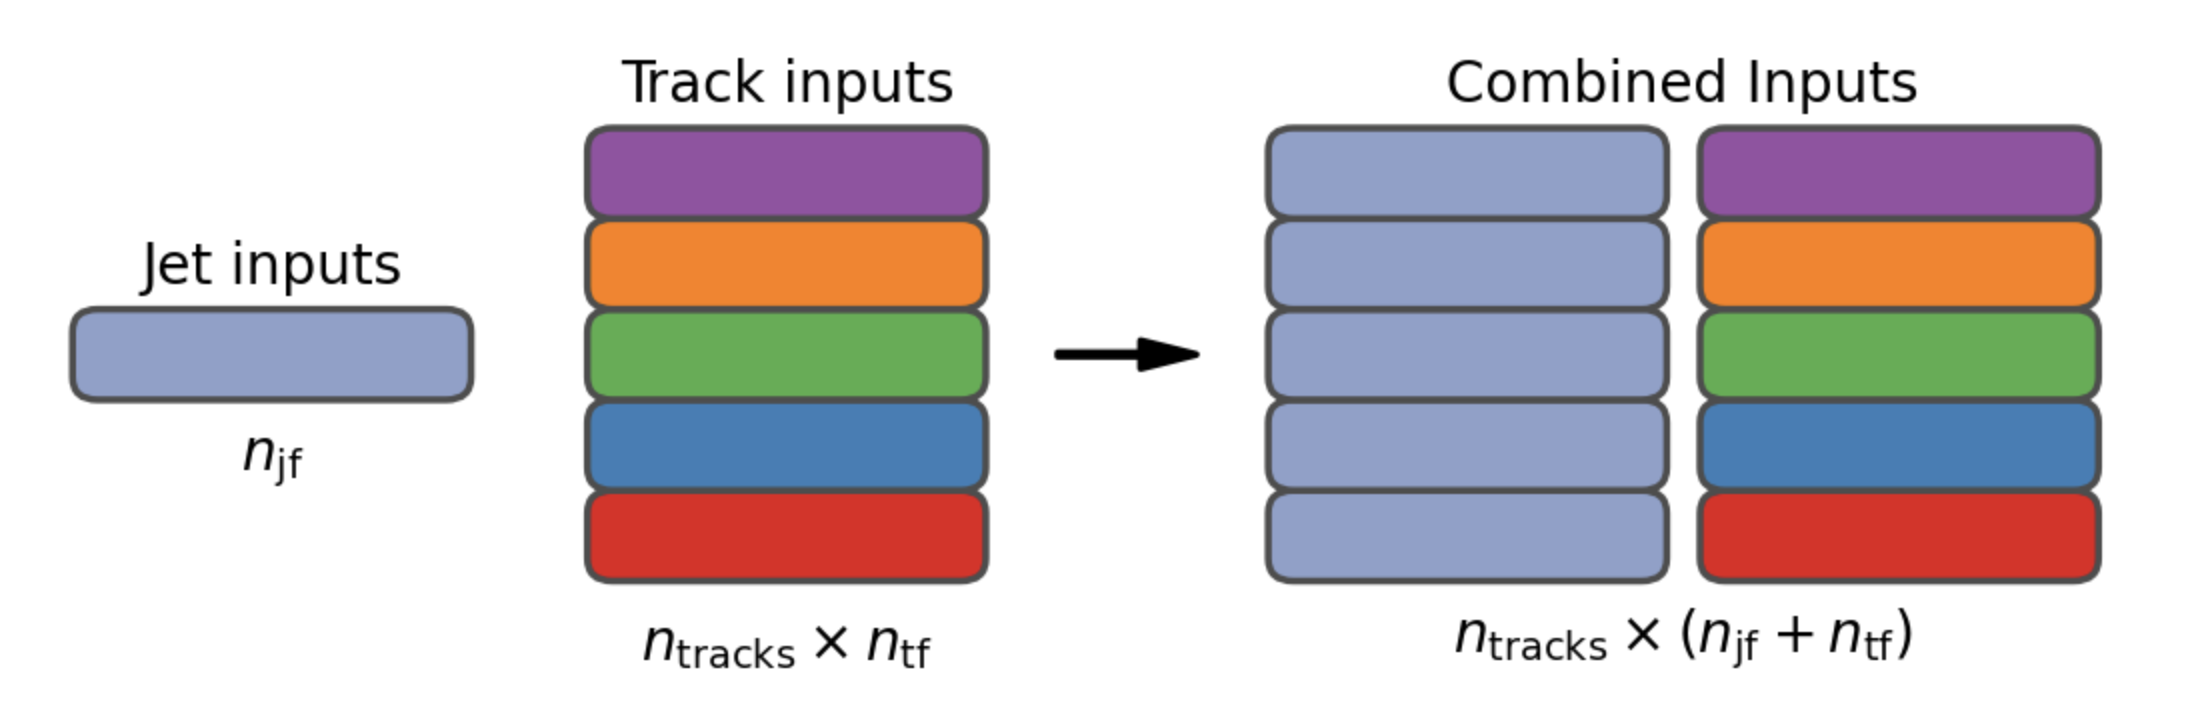
\includegraphics[width=0.6\textwidth]{chapters/gnn_tagger/figs/inputs_diagram.png}
    \caption{The inputs to \GNN are the two jet features ($n_\text{jf} = 2$), and an array of $n_{\text{tracks}}$, where each track is described by 21 track features ($n_\text{tf} = 21$) \cite{ATL-PHYS-PUB-2022-027}. The jet features are copied for each of the tracks, and the combined jet-track vectors of length 23 form the inputs of \GNN.}
    \label{fig:model_input_array}
\end{figure}

\begin{figure}[!htbp]
    \centering
    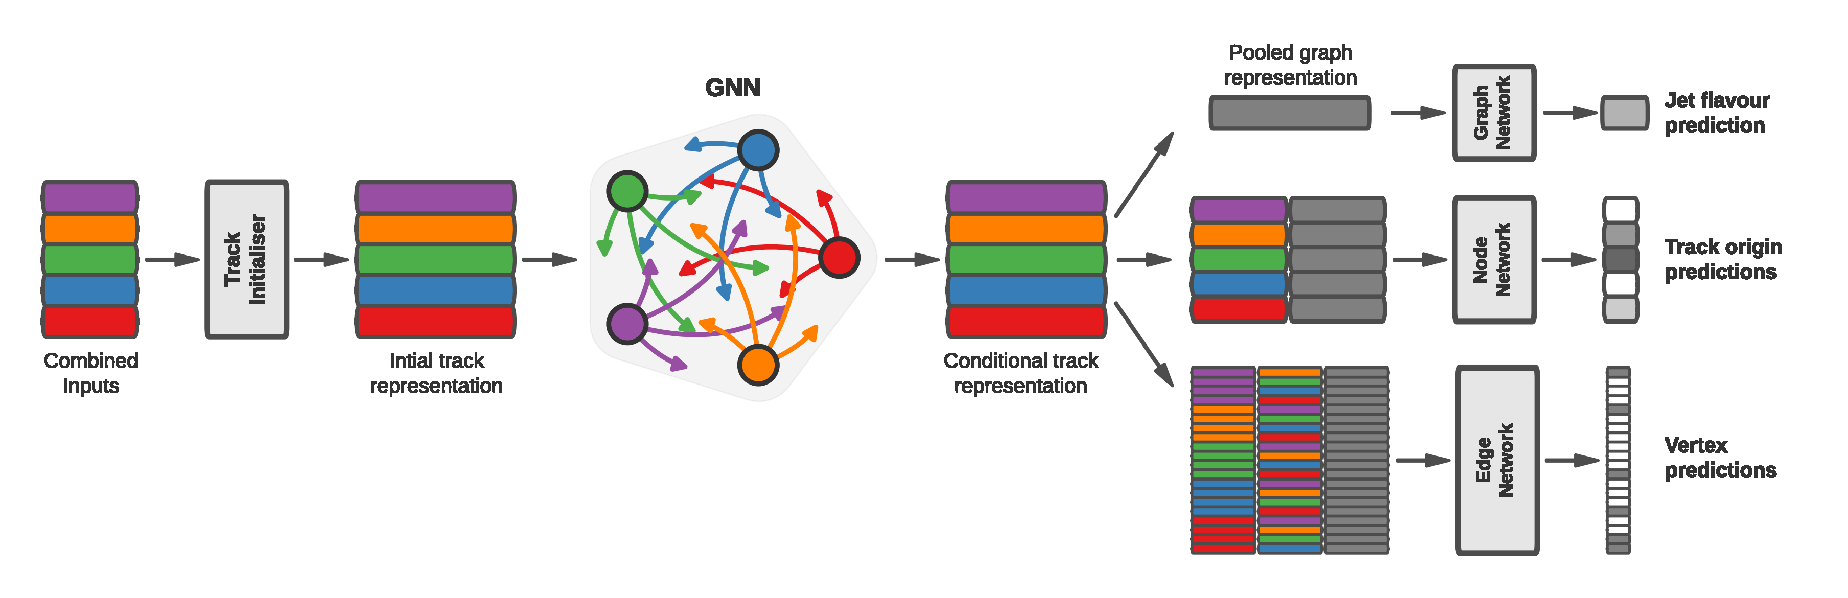
\includegraphics[width=\textwidth]{chapters/gnn_tagger/figs/full_arch.pdf}
    \caption{The network architecture of \GNN. Inputs are fed into a per-track initialisation network, which outputs an initial latent representation of each track. These representations are then used to populate the node features of a fully connected graph network. After the graph network, the resulting node representations are used to predict the jet flavour, the track origins, and the track-pair vertex compatibility.}
    \label{fig:new_arch}
\end{figure}

The outputs of the track initialisation network are used to populate the nodes of a fully connected graph, such that each node in the graph neighbours every other node.
Each node $h_i$ in the graph corresponds to a single track in the jet, and is characterised by a feature vector, also called a representation.
The per-track output representations from the initialisation networks are used as the initial feature vectors of each node in the graph.
In each layer of the graph network, output node representations $h_i'$ are computed by aggregating the features of $h_i$ and neighbouring nodes $\mathcal{N}_i$ using a multi-head attention mechanism ($n=2$) as described in Ref.~\cite{2021arXiv210514491B,2017arXiv170603762V}.
First, the feature vectors of receiver and sender nodes are fed into two fully connected linear layers $\mathbf{W}_r$ and $\mathbf{W}_s$, to produce an updated representation for each sender and receiver node $\mathbf{W}_r h_i$ and $\mathbf{W}_s h_j$.
These updated feature vectors are used to compute edge scores $e(h_i, h_j)$ for each node pair, as in

\begin{equation}\label{eq:edge_score}
    e(h_i, h_j) = \mathbf{a} \cdot \theta \left[ \mathbf{W}_r h_i + \mathbf{W}_s h_j \right],
\end{equation}

where, $\theta$ is a non-linear activation function, and $\mathbf{a}$ is a learned vector.
These edge scores are then used to calculate attention weights $a_{ij}$ for each pair of nodes using the softmax function over the edge scores

\begin{equation}\label{eq:attention weights}
    a_{ij} = \mathrm{softmax}_j \left[ e(h_i, h_j) \right].
\end{equation}

Finally, the updated representations for the receiver nodes $h_i'$ are computed by taking the weighted sum over each updated node representation $\mathbf{W}_r h_i$, with weights $a_{ij}$

\begin{equation}\label{eq:updated_node_rep}
    h'_i = \sigma \left[ \sum_{j \in \mathcal{N}_i}{a_{ij} \cdot \mathbf{W}_r {h}_j}  \right].
\end{equation}

The set of operations described above constitute a single graph network layer. 
Three such layers are stacked to construct the graph network, representing a balance between achieving good performance in a reasonable time and avoiding overtraining due to inflation of the parameter count of the model.
The final output from the graph neural network is a set of per-node (i.e. per-track) feature vectors that are conditional representations of each track given the other tracks in the jet.
In order to perform the jet flavour prediction, a flattened global representation of the jet is needed.
To produce this, the output track representations are combined using a weighted sum, where the weights are learned during training and therefore act as a form of attention over the different tracks.
The flattened outputs from the sum are then fed into a fully connected feedforward neural network with four layers and three outputs, one for each jet flavour.
Two other separate fully connected feedforward neural networks are then also used to independently perform the auxiliary classification objectives of \GNN.
Both of the auxiliary classification tasks also take in the global representation of the jet as inputs.
A summary of the different classification networks used for the various training objectives is shown in \cref{tab:architecture}.

\begin{table}[!htbp]
  \footnotesize\centering
  \setlength{\tabcolsep}{0.5em} % for the horizontal padding
  \begin{tabular}{llll}
      \toprule\hline 
      \textbf{Network} & \textbf{Hidden layers} & \textbf{Output size} & \textbf{Label} \\
      \hline
      Node classification network    & 128, 64, 32 & 7 & Track origin \\
      Edge classification network    & 128, 64, 32 & 1 & Track-pair compatability \\
      Graph classification network   & 128, 64, 32, 16 & 3 & Jet flavour \\
      \hline\bottomrule
  \end{tabular}
  \caption{
    A summary of GN1's different classification networks used for the various training objectives, adapted from \rcite{ATL-PHYS-PUB-2022-027}.
    The hidden layers column contains a list specifying the number of neurons in each layer.
  }
  \label{tab:architecture}
\end{table}

The node classification network predicts the track truth origin as defined in~\cref{tab:truth_origins}.
This network takes as inputs the features from a single output node from the graph network and the global representation of the jet.
The node network has three hidden layers containing 128, 64 and 32 neurons respectively, and an output size of seven, corresponding to the seven different truth origins defined in~\cref{tab:truth_origins}.

The edge classification network is used to predict whether the tracks in the track-pair belong to a common vertex.
This network takes as inputs the concatenated representations from each pair of tracks and the global jet representation.
Similar to the node network, the edge network has three hidden layers containing 128, 64 and 32 neurons respectively, and a single output, which is used to perform binary classification of the track-pair compatability.
The output predictions for the two auxiliary networks are used for the auxiliary training objectives discussed in \cref{sec:aux-train-objectives}.

Finally, the graph classification network is used to predict the jet flavour.
This network takes only the global jet representation as input.
The graph classification network is comprised of four fully connected hidden layers with 128, 64, 32 and 16 neurons respectively, and has three outputs corresponding to the \bcl jet classes. 



\subsection{Training}\label{sec:training}

The full \GNN training procedure minimises the total loss function $L_\text{total}$, defined in \cref{eq:loss}. 
This loss is composed of three terms: $L_\text{jet}$, the categorical cross entropy loss over the different jet flavours; $L_\text{vertex}$, the binary track-pair compatability cross entropy loss; and $L_\text{track}$, the categorical cross entropy loss for the track origin prediction.
$L_\text{vertex}$ is computed via a weighted average over all intra-jet track-pairs in the batch, and $L_\text{track}$ is computed by a weighted average over all tracks in the batch, where the weights are described below.

\begin{equation}\label{eq:loss}
    L_\text{total} = L_\text{jet} + \alpha L_\text{vertex} + \beta L_\text{track}
\end{equation}

The different losses converge to different values during training, reflecting differences in the relative difficulty of the various training objectives.
The values of $L_\text{vertex}$ and $L_\text{track}$ are weighted by $\alpha = 1.5$ and $\beta = 0.5$ respectively to ensure they converge to similar values, giving them an equal weighting towards $L_\text{total}$. 
The values of $\alpha$ and $\beta$ are chosen to ensure that $L_\text{jet}$ converges to a larger value than either $L_\text{vertex}$ and $L_\text{track}$, which reflects the primary importance of the jet classification objective.
It was found that in practice the overall performance of the model was not sensitive to modest changes in the loss weights $\alpha$ and $\beta$.
Pre-training using $L_\text{total}$ (i.e. on all tasks) and fine tuning on only the jet classification task also did not improve performance versus the described standard setup, indicating that the auxiliary tasks are not in direct competition with the jet classification task.
As there was a large variation in the relative abundance of tracks of the different origins, the contribution of each origin to $L_\text{track}$ was weighted by the inverse of the frequency of their occurrence.
In vertexing loss $L_\text{vertex}$, the class weight for track-pairs where both tracks are from either a \borchadron was increased by a factor of two as compared with other track-pairs, to encourage the network to focus on correctly classifying heavy flavour vertices.

\GNN can be trained with either the node or edge networks (and their corresponding auxiliary tasks), or both, removed, as discussed in \cref{sec:gnn_ablations}.
In such cases, the corresponding losses $L_\text{vertex}$ and $L_\text{track}$ are also removed from the calculation of the overall loss $L_\text{total}$. 
The performance of the resulting models provides a useful indication of the benefit of including the auxiliary tasks to the primary jet classification objective.

\GNN was trained for \nepochs epochs on 4 NVIDIA V100 GPUs.
Each epoch takes approximately \minsperepoch mins to complete over the training sample of \njetstrain jets described in \cref{sec:datasets}.
The Adam optimiser~\cite{arxiv.1412.6980} with an initial learning rate of $1\mathrm{e}{-3}$, and a batch size of 4000 jets (spread across the 4 GPUs) was used.
Typically the validation loss, calculated on \njetsval jets, became stable after around 60 epochs.
The epoch that minimized the validation loss was used for evaluation.
\GNN has been integrated into the ATLAS software~\cite{ATL-SOFT-PUB-2021-001} using ONNX~\cite{bai2019}.
The test sample jet flavour predictions scores are computed using the ATLAS software stack as a verification of this process.
%\todo{inlcude loss vs epoch? or save for paper}


\section{Results}\label{sec:gnn_results}


The \GNN tagger is evaluated both as a \btag and \ctag algorithm in \cref{sec:gnn_btag_perf} and \cref{sec:gnn_ctag_perf} respectively.
Evaluation is performed separately on both \ttbarjets with \ttbarpt and \Zprimejets with \Zprimept.
The performance of the model is compared to the \DLr tagger~\cite{ATL-PHYS-PUB-2017-013,ATLAS:2022qxm}, which has been retrained on 75 million jets from the same samples as \GNN.
The input RNNIP tagger~\cite{ATL-PHYS-PUB-2017-003} to \DLr has not been retrained.
As discussed, each tagger predicts the probability that a jet belongs to the \bcl classes.
To use the model for \btag, these probabilities are combined into a single score \Db, which is defined as
%\DLr is a modification of the previous \DLr tagger \cite{ATL-PHYS-PUB-2017-013} which which replaces RNNIP with DIPS, a separately trained track-based algorithm based on deep sets. 
%The DIPS tagger uses the loose track selection defined in \cite{ATL-PHYS-PUB-2020-014}.

\begin{equation}\label{eq:btag-disc}
    \Db = \log{\frac{p_b}{(1-\fc )p_l + \fc  p_c}} ,
\end{equation}

where \fc is a free parameter that determines the relative weight of $p_c$ to $p_l$ in the score \Db, controlling the trade-off between $c$- and \lrej performance.
The choice of \fc is arbitrary, and is optimised based upon the desired light- vs \cjet rejection performance.
This parameter is set to a value of $\fc = 0.018$ for the \DLr model, obtained through an optimisation procedure described in \rcite{ATL-PHYS-PUB-2017-013}.
Based on a similar optimisation procedure, a value of $\fc = 0.05$ is used for the \GNN models.
A fixed-cut working point (WP) defines the corresponding selection applied to the tagging discriminant \Db in order to achieve a given efficiency on the inclusive \ttbar sample.

%The technical implementation of \GNN in the ATLAS software stack requires any jet with zero or one associated tracks to be classified as a \ljet.
%The impact of this on the tagging performance of \GNN was found to be negligible, with \pct{0.12} of \ttbarbjets and \pct{0.02} of \Zprimebjets affected.
%Of those, \pct{89} of the \ttbarbjets and \pct{98} of the \Zprimebjets are also classified as \ljets by \DLr at the \pct{70} \ttbar WP.

A comparison of the \btag discriminant \Db between \DLr and \GNN is shown in \cref{fig:ttbar_btag_disc}. 
The shapes of the \Db distributions are generally similar for \bcl jets between both models, however, \GNN shifts the \bjet distribution to higher values of \Db in the regions with the greatest discrimination.
The \GNN \cjet distribution is also shifted to lower values of \Db when compared with \DLr, enhancing the separation and indicating that \GNN is improving \cjet rejection when compared with \DLr.

\begin{figure}[!htb]
    \centering
    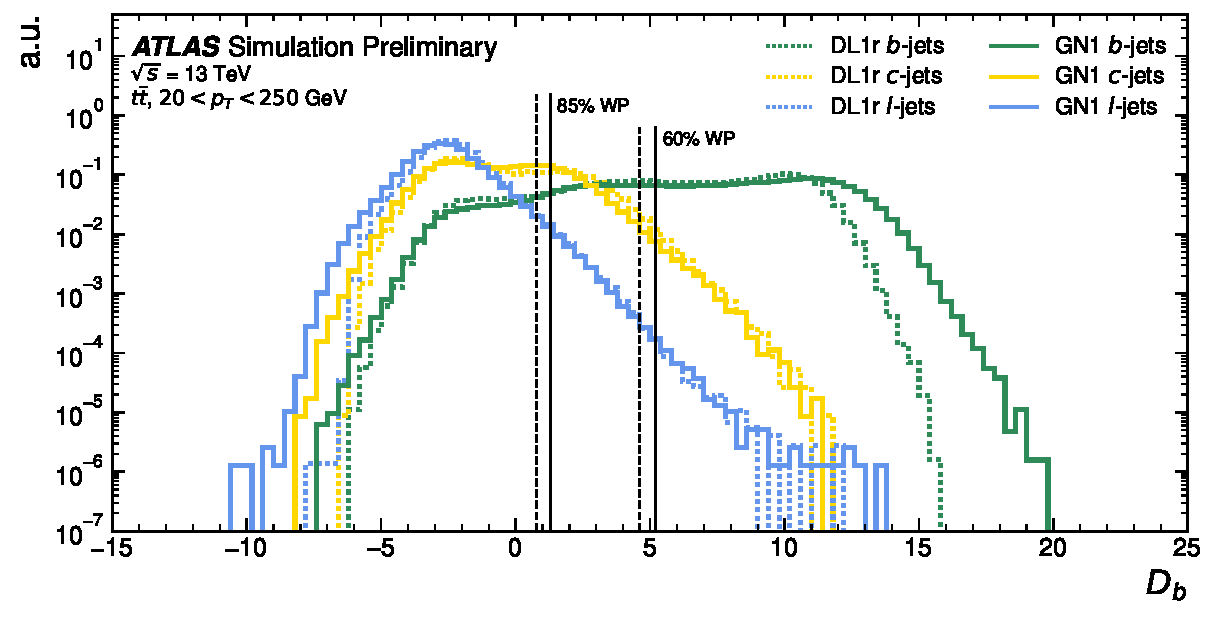
\includegraphics[width=0.8\textwidth]{chapters/gnn_tagger/figs/results/main/ttbar/ttbar_score_DL1r_GN120220509_btag.pdf}
    \caption{Comparison between the \DLr and \GNN \btag discriminant \Db for jets in the \ttbar sample \cite{ATL-PHYS-PUB-2022-027}.
    The \pct{85} WP and the \pct{60} WP are marked by the solid (dashed) lines for \GNN (\DLr), representing respectively the loosest and tightest WPs typically used by analyses.
    A value of $\fc = 0.018$ is used in the calculation of \Db for \DLr and $\fc = 0.05$ is used for \GNN. The distributions of the different jet flavours have been normalised to unity area.}
    \label{fig:ttbar_btag_disc}
\end{figure}



\subsection{\texorpdfstring{\btagging}{b-tagging} Performance}\label{sec:gnn_btag_perf}

The performance of \btag algorithms is quantified by their ability to reject \cljets for a given \bjet selection efficiency WP.
In order to compare the \btag performance of the different taggers for the \bjet tagging efficiencies in the range typically used by analyses, the corresponding \clrej rates are displayed in \cref{fig:ttbar_btag_roc,fig:zprime_btag_roc} for jets in the \ttbar and \Zprime samples respectively.
Four standard WPs are defined with \bjet tagging efficiencies of \pct{60}, \pct{70}, \pct{77} and \pct{85} respectively.
These WPs are commonly used by physics analyses depending on their specific signal and background requirements.
The WPs are defined based on \ttbarjets only.
Due to the much higher jet \pt range in the \Zprime sample, and the increased difficulty in tagging jets at \highpt (see \cref{chap:tracking}), the \bjet tagging efficiencies for \Zprimejets are lower than the corresponding WPs calculated in the \ttbar sample.
For instance the WP cut value computed to provide a $70\%$ \bjet tagging efficiency on the \ttbar sample results in a \bjet tagging efficiency of just $\sim30\%$ on the \Zprime sample.
In order to account for this, the range of \bjet tagging efficiencies displayed for plots showing the performance for \Zprimejets (for example \cref{fig:zprime_btag_roc}) is chosen to span the lower efficiencies achieved in the \Zprime sample at \highpt.

For \ttbarjets with \ttbarpt, \GNN demonstrates considerably better \clrej when compared with \DLr across the full range of \bjet tagging efficiencies studied.
The relative improvement is strongly dependent on the \bjet tagging efficiency under study.
The largest improvements are found at lower \bjet tagging efficiencies.
At a \bjet tagging efficiency of \pct{\ttlo}, the \crej improves by a factor of \ttbclo while the \lrej improves by a factor of \ttbllo with respect to \DLr.
For \highpt \Zprimejets with \Zprimept, \GNN also brings a significant performance improvement with respect to \DLr across the range of \bjet tagging efficiencies studied.
Again, the largest relative improvement in performance comes at the lower \bjet tagging efficiencies.
At a \bjet efficiency of \pct{\zplo}, \GNN improves the \crej with respect to \DLr by a factor of \zpbclo and the \lrej by a factor of \zpbllo.
The performance comparison at lower \bjet tagging efficiencies is made more difficult due to the increased statistical uncertainties which result from the high rejection of background.
%It is estimated that for a \bjet tagging efficiency of $70\%$ in the \ttbar sample, $\sim5\%$ ($\sim30\%$) of the relative improvement in the \cjet (\ljet) rejection comes from loosening the track selection and for a \bjet tagging efficiency of $30\%$ in the \Zprime the corresponding number is $\sim10\%$ for both \cjets and \ljets.
Given that \GNN exploits the low-level detector information in a more complete and sophisticated way than \DLr, further studies are needed to confirm that the performance gain observed in these simulated samples is also observed in experimental data.

The \GNNLep variant of \GNN demonstrates further improved performance with respect to the baseline model.
This demonstrates the additional jet flavour discrimination power provided by the leptonID track input.
For \ttbarjets, the relative \crej improvement with respect to \GNN at the \bWP{\ttlo} is approximately \pct{30}.
The improvement in \lrej also increases by \pct{40} at the same WP.
For \Zprimejets, the relative \crej (\lrej) performance with respect to \GNN improves by approximately \pct{10} (\pct{25}) at a \bjet tagging efficiency of \pct{\zplo}.
%As shown in \cref{fig:vs_pt_flat_leff}, the greatest improvement of \GNNLep over \GNN is seen at lower transverse momenta.

\begin{figure}[!p]
    \centering
    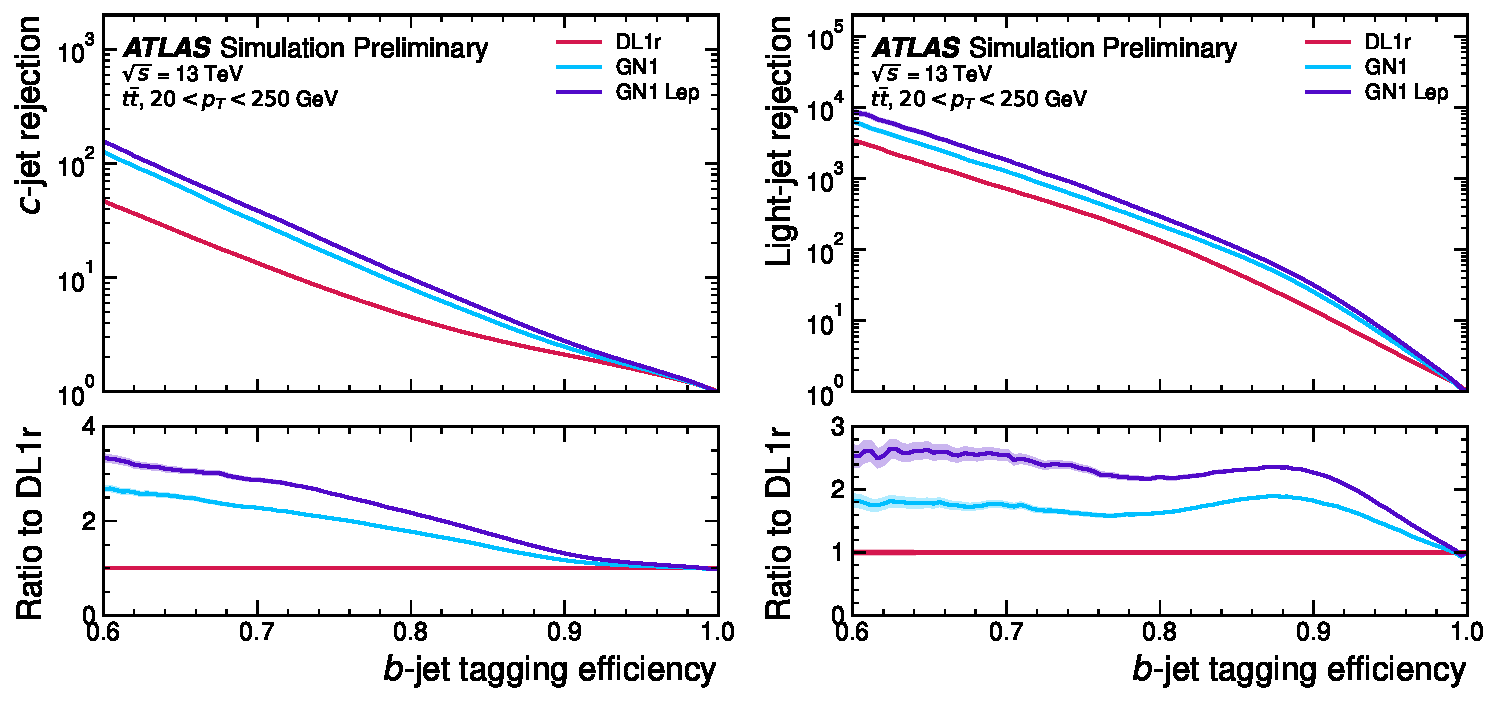
\includegraphics[width=\textwidth]{chapters/gnn_tagger/figs/results/main/ttbar/ttbar_roc_btag.pdf}
    \caption{The \cjet (left) and \ljet (right) rejections as a function of the \bjet tagging efficiency for \ttbarjets with \ttbarpt \cite{ATL-PHYS-PUB-2022-027}.
             The ratio with respect to the performance of the \DLr algorithm is shown in the bottom panels.
             A value of $\fc = 0.018$ is used in the calculation of \Db for \DLr and $\fc = 0.05$ is used for \GNN and \GNNLep.
             Binomial error bands are denoted by the shaded regions.
             The $x$-axis range is chosen to display the \bjet tagging efficiencies usually probed in these regions of phase space.}
    \label{fig:ttbar_btag_roc}
\end{figure}

\begin{figure}[!p]
    \centering
    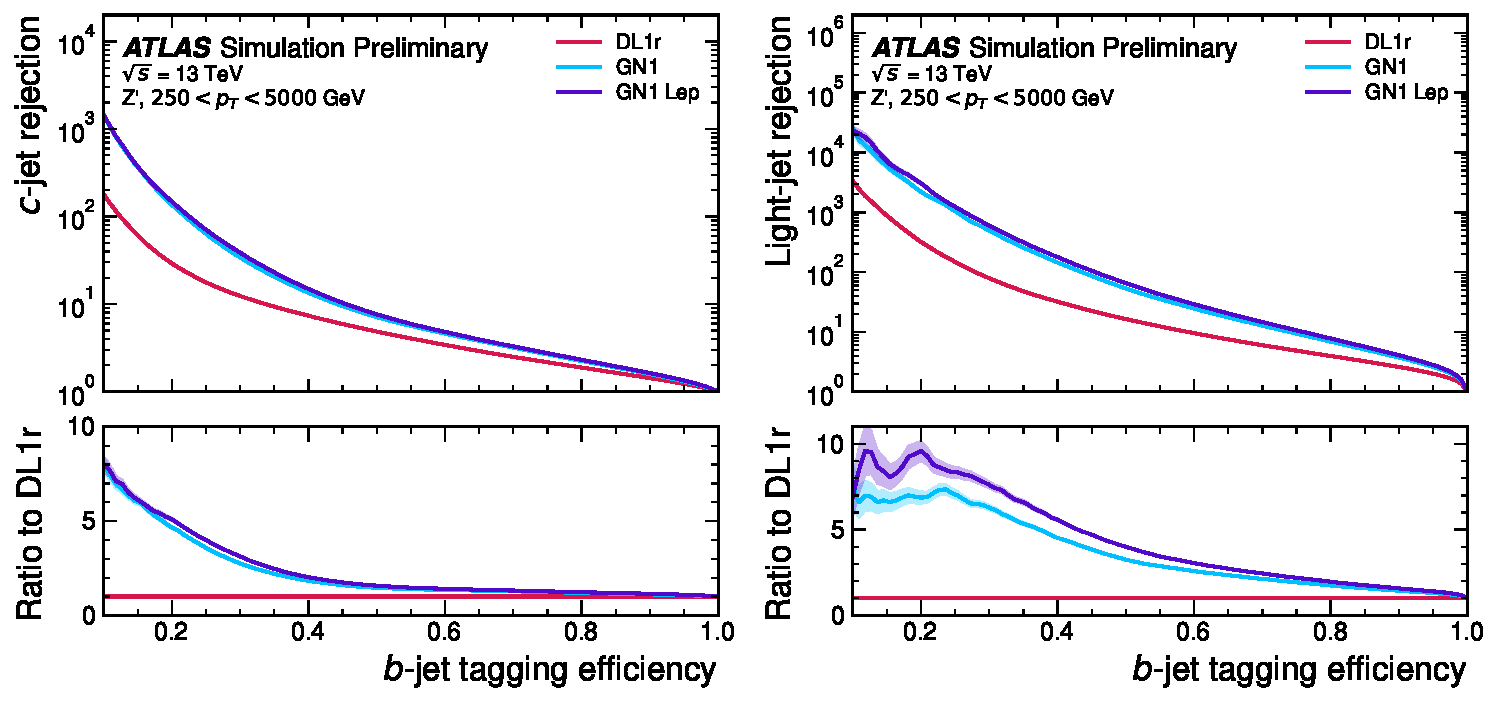
\includegraphics[width=\textwidth]{chapters/gnn_tagger/figs/results/main/zprime/zprime_roc_btag.pdf}
    \caption{The \cjet (left) and \ljet (right) rejections as a function of the \bjet tagging efficiency for \Zprimejets with \Zprimept \cite{ATL-PHYS-PUB-2022-027}.
             The ratio with respect to the performance of the \DLr algorithm is shown in the bottom panels.
             A value of $\fc = 0.018$ is used in the calculation of \Db for \DLr and $\fc = 0.05$ is used for \GNN and \GNNLep.
             Binomial error bands are denoted by the shaded regions.
             The $x$-axis range is chosen to display the \bjet tagging efficiencies usually probed in these regions of phase space.}
    \label{fig:zprime_btag_roc}
\end{figure}

In general, the performance of all the taggers is strongly dependent on the jet \pt.
This is due to the increased multiplicity and collimation of tracks, and the displaced decays that result from within the heavy flavour jets (see \cref{chap:tracking}).
Together, they contribute to a reduced reconstruction efficiency for heavy flavour tracks, and a general degradation in quality of tracks inside the core of a jet, which in turn reduces the jet tagging performance.

In order to study how the tagging performance changes as a function of the jet \pt, the \bjet tagging efficiency as a function of \pt for a fixed \ljet rejection of 100 in each bin is shown in \cref{fig:vs_pt_flat_leff}.
For \ttbarjets, at a fixed \ljet rejection of 100, \GNN improves the \bjet tagging efficiency by approximately \pct{4} across all the jet \pt bins.
Meanwhile, \GNNLep again demonstrates improved performance with respect to \GNN, in particular at lower \pt.
The relative increase in the \bjet tagging efficiency increases from \pct{4} to \pct{8} with respect to \DLr.
For \Zprimejets, \GNN again outperforms \DLr across the entire jet \pt range studied.
The largest relative improvement in performance is found at the highest transverse momenta of jet $\pt > \SI{2}{\TeV}$, and corresponds to an approximate factor of 2 improvement in efficiency with respect to \DLr.

The performance of the model was also evaluated as a function of the average number of pileup interactions in the event. No significant dependence of the tagging performance was observed.


\begin{figure}[!htbp]
    \centering
    \begin{subfigure}[b]{0.48\textwidth}
        \centering
        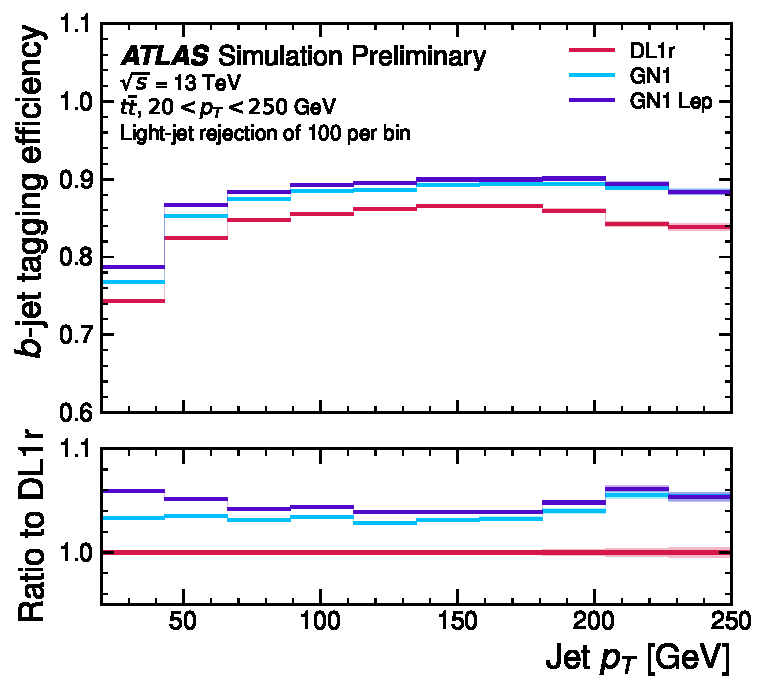
\includegraphics[width=\textwidth]{chapters/gnn_tagger/figs/results/main/ttbar/ttbar_flat_leff_by_pt_btag.pdf}
        %\caption{sub}
        %\label{fig:sub}
    \end{subfigure}
    \quad
    \begin{subfigure}[b]{0.48\textwidth}
        \centering
        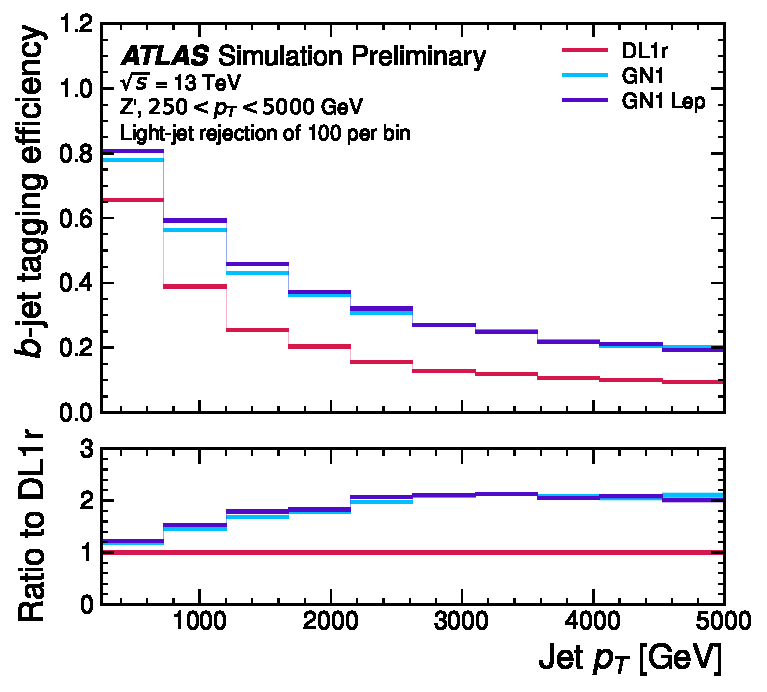
\includegraphics[width=\textwidth]{chapters/gnn_tagger/figs/results/main/zprime/zprime_flat_leff_by_pt_btag.pdf}
        %\caption{sub}
        %\label{fig:sub}
    \end{subfigure}
    \caption{The \bjet tagging efficiency for \ttbarjets (left) and \Zprimejets (right) as a function of jet \pt with a fixed \ljet rejection of 100 in each bin \cite{ATL-PHYS-PUB-2022-027}.
             %For \ttbarjets, \GNN increases \beff by approximately \pct{5} with respect to \DLr in each \pt bin.
             %For \Zprimejets, \GNN increases \beff by up to a factor of 2 for jets with $\pt > \SI{2.5}{\TeV}$ with respect to \DLr.
             A value of $\fc = 0.018$ is used in the calculation of \Db for \DLr and $\fc = 0.05$ is used for \GNN and \GNNLep.
             \GNN demonstrates improved performance with respect to \DLr accross the \pt range shown.
             Binomial error bands are denoted by the shaded regions.
             }
    \label{fig:vs_pt_flat_leff}
\end{figure}




\subsection{\texorpdfstring{\ctagging}{c-tagging} Performance}\label{sec:gnn_ctag_perf}

As discussed previously, \GNN does not rely on any inputs from manually optimised low-level tagging algorithms.
Since these algorithms were originally designed and tuned with the aim of \btag, and not \ctag, the low level tagging algorithms may perform suboptimally for \ctag purposes.
The tagging of \cjets therefore presents a compelling use case for \GNN.
As each of the the models is trained with three output classes, using it as a \ctagging algorithm is trivially analogous to the approach used for \btag.
The model output probabilities are combined into a single score \Dc, which is defined similarly to \cref{eq:btag-disc} as

\begin{equation}\label{eq:ctag-disc}
    D_c = \log{\frac{p_c}{(1-f_b)p_l + f_b p_b}} .
\end{equation}

A value of $\fb = 0.2$ is used for all models, based on the same optimisation procedure that was used for the \btag use case.
Similar to \cref{sec:gnn_btag_perf}, the different taggers are compared to one another by scanning through a range of \cjet tagging efficiencies and plotting the corresponding \blrej rates.
As in \cref{sec:gnn_btag_perf}, the WPs are defined using \ttbarjets.
Standard \cjet tagging efficiency WPs used by physics analyses are significantly lower than the \btag WPs in order to maintain reasonable $b$- and \ljet rejection rates.
This is reflected in the range of \cjet tagging efficiencies used in \ctag plots such as \cref{fig:ttbar_ctag_roc,fig:zprime_ctag_roc}.
\cref{fig:ttbar_ctag_roc} displays the \ctag performance of the models on the \ttbarjets.
\GNN is shiown to perform significantly better than \DLr.
Similar to the \btag case, the \blrej improve most at lower \cjet tagging efficiencies, with the \crej (\lrej) improving by a factor $2$ ($1.6$) with respect to \DLr at a \cjet tagging efficiency of \pct{25}.
\GNNLep again outperforms \GNN, though the improvements are more modest than observed for the \btag use case, with the both the \brej and \lrej improving with respect to \GNN by approximately \pct{10} at the \WP{25}{c}.
\cref{fig:zprime_ctag_roc} shows the \ctag performance on the \Zprimejets with \Zprimept.
Both \GNN and \GNNLep perform similarly, improving the \brej by \pct{60} and the \lrej by a factor of 2 at the \WP{25}{c}.

\begin{figure}[!p]
    \centering
    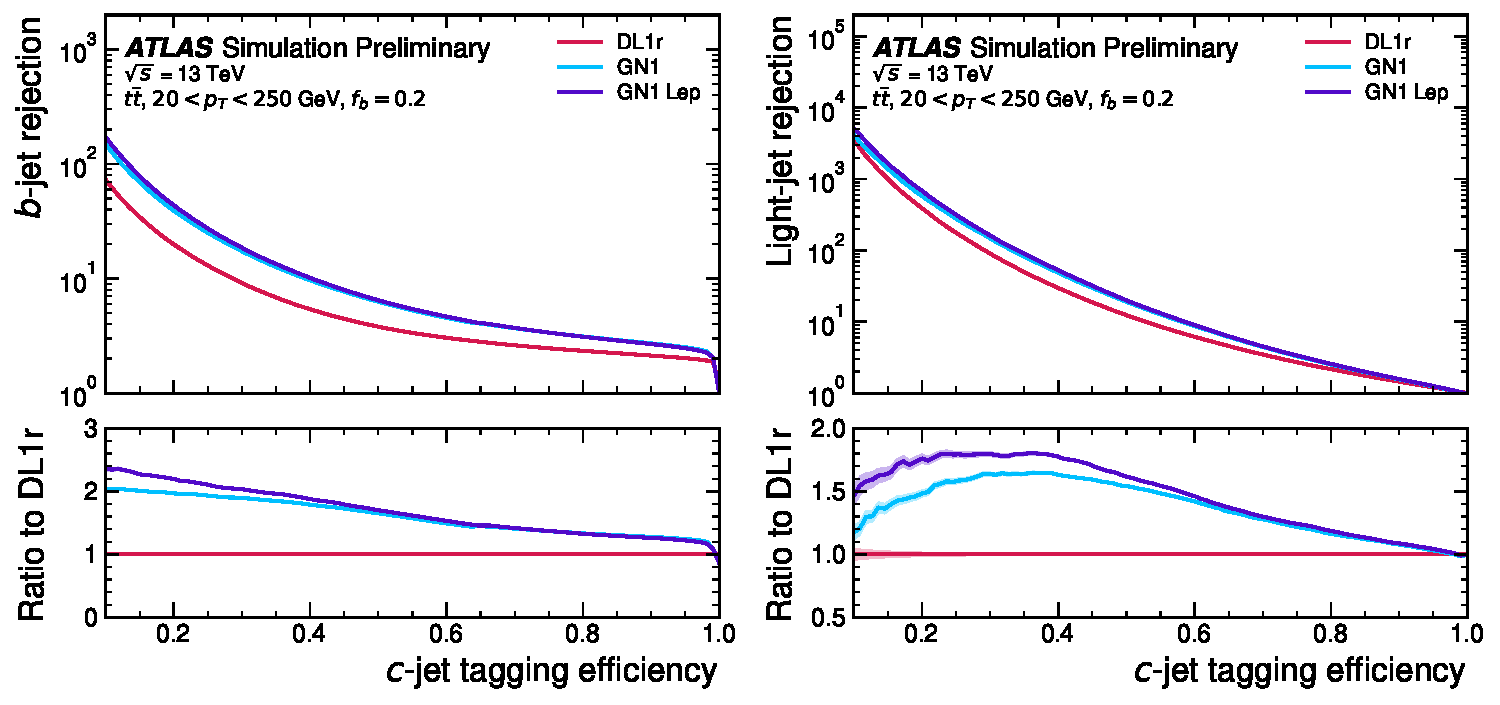
\includegraphics[width=\textwidth]{chapters/gnn_tagger/figs/results/main/ttbar/ttbar_roc_ctag.pdf}
    \caption{
        The \bjet (left) and \ljet (right) rejections as a function of the \cjet tagging efficiency for \ttbar jets with \ttbarpt \cite{ATL-PHYS-PUB-2022-027}.
        The ratio to the performance of the \DLr algorithm is shown in the bottom panels.
        Binomial error bands are denoted by the shaded regions.
        The $x$-axis range is chosen to display the \cjet tagging efficiencies usually probed in these regions of phase space.
    }
    \label{fig:ttbar_ctag_roc}
\end{figure}

\begin{figure}[!p]
   \centering
   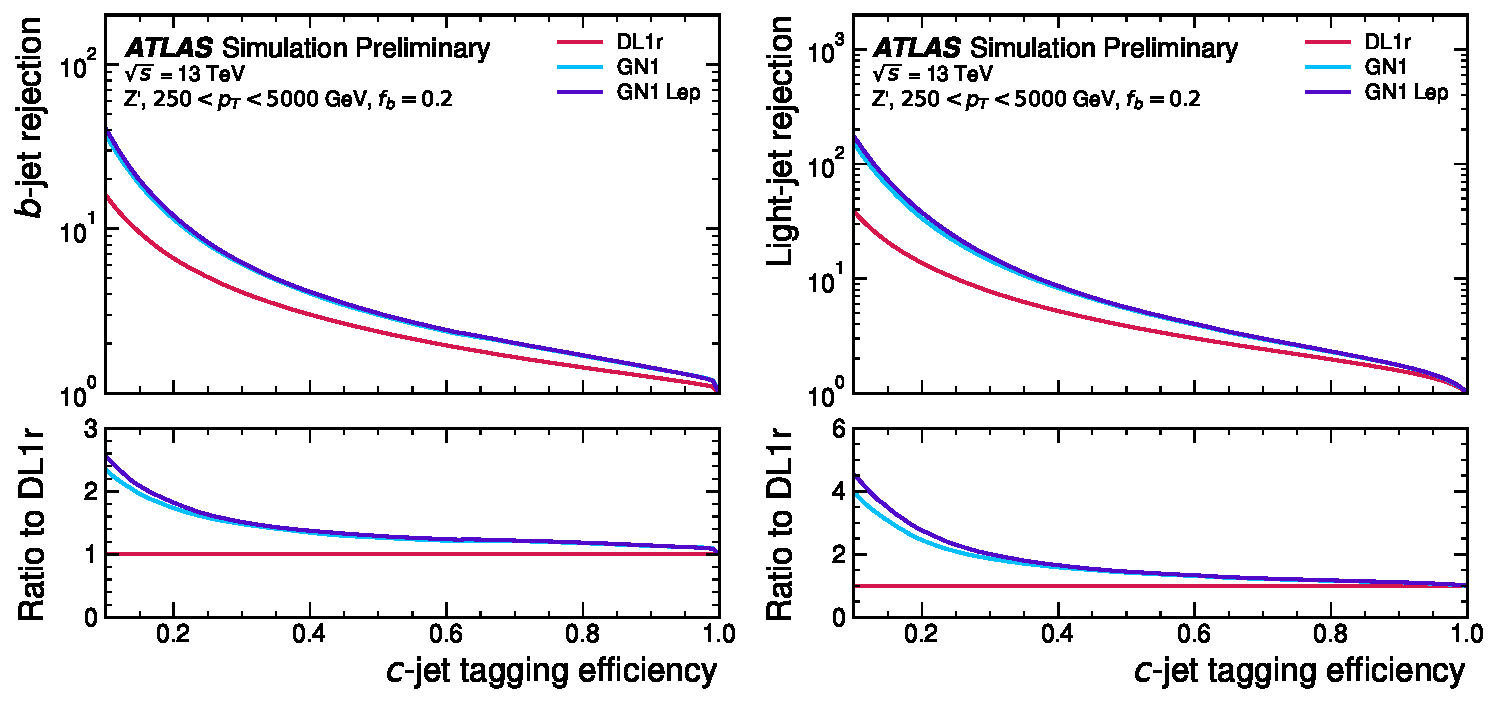
\includegraphics[width=\textwidth]{chapters/gnn_tagger/figs/results/main/zprime/zprime_roc_ctag.pdf}
   \caption{
        The \bjet (left) and \ljet (right) rejections as a function of the \cjet tagging efficiency for \Zprime jets with \Zprimept \cite{ATL-PHYS-PUB-2022-027}.
        The ratio to the performance of the \DLr algorithm is shown in the bottom panels.
        Binomial error bands are denoted by the shaded regions.
        The $x$-axis range is chosen to display the \cjet tagging efficiencies usually probed in these regions of phase space.
    }
   \label{fig:zprime_ctag_roc}
\end{figure}




\subsection{Ablations}\label{sec:gnn_ablations}

Ablation studies (the removal of certain components of a given model in order to study the impact of that component) are carried are carried out to determine the importance of the auxiliary training objectives of \GNN to the overall performance.
The ``\GNN No Aux'' variant retains the primary jet classification objective, but removes both track classification and vertexing auxiliary objectives (see \cref{sec:aux-train-objectives}) and correspondingly only minimises the jet classification loss.
The ``\GNN TC'' variant includes track classification objective but not the vertexing objective.
Finally, the ``\GNN Vert'' includes the vertexing objective, but not the track classification objective.

For jets in both the \ttbar and \Zprime samples, a general trend is observed that the models trained without one or both of the auxiliary objectives results in significantly reduced \clrej when compared with the baseline \GNN model.
This result is shown clearly in \cref{fig:ttbar_btag_roc_ab,fig:zprime_btag_roc_ab}.
For \ttbarjets, the performance of \GNN No Aux is similar to \DLr, while \GNN TC and \GNN Vert perform similarly to each other.
For \Zprimejets meanwhile, the \GNN No Aux model already shows a clear improvement in \clrej when compared with \DLr at lower \bjet tagging efficiencies.
Similar to \ttbarjets, \GNN TC and \GNN Vert perform similarly, and bring large gains in background rejection when compared with \GNN No Aux, but the combination of both auxiliary objectives yields the best performance.

It is notable that the \GNN No Aux model matches or exceeds the performance of \DLr without the need for inputs from the low-level algorithms.
This indicates that the performance improvements enabled by the improved neural network architecture used in \GNN appear to be able to compensate for the removal of the low-level algorithm inputs.
The \GNN TC and \GNN Vert variants each similarly outperform \DLr, demonstrating that both contribute to the overall high performance of the baseline model.
The overall best performing model is the full version of \GNN trained with both auxiliary objective, demonstrating that the two auxiliary objectives are complementary.

\begin{figure}[!p]
    \centering
    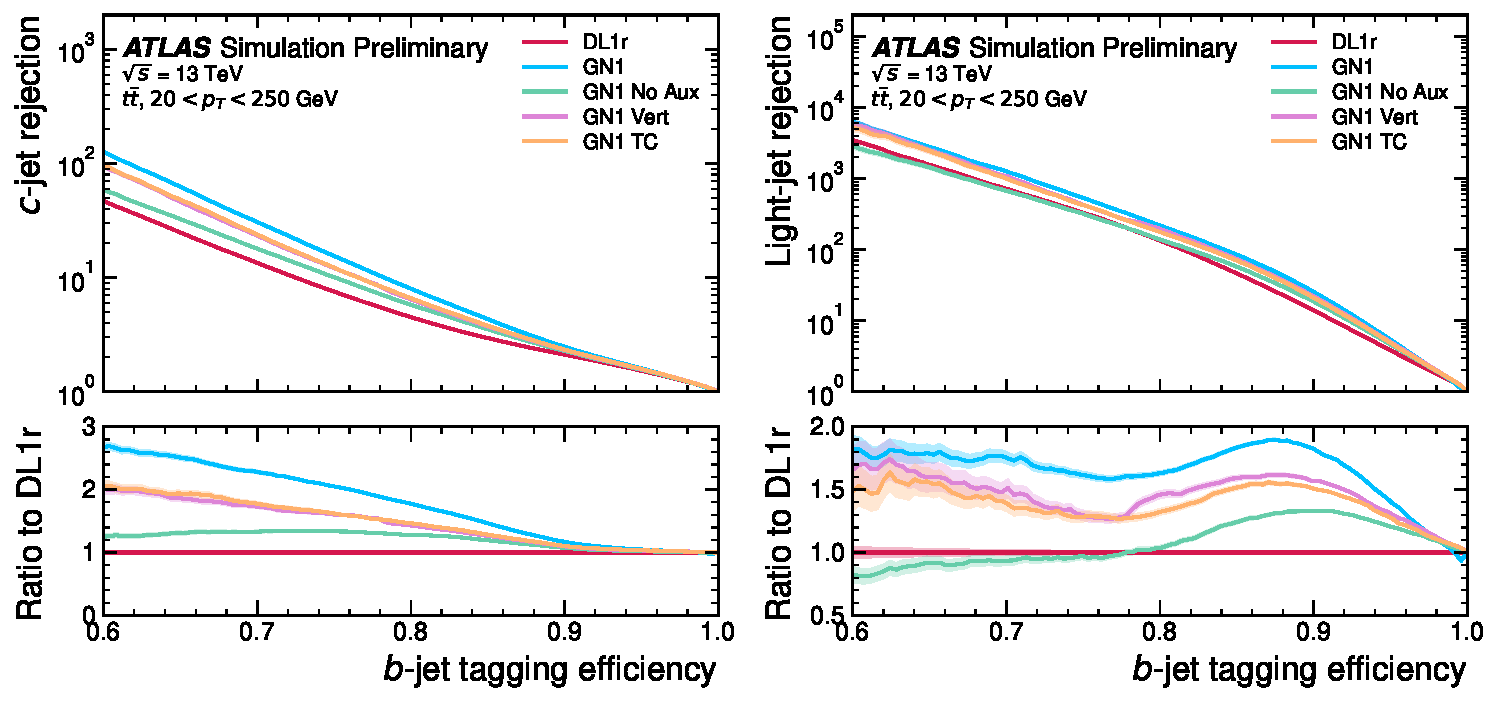
\includegraphics[width=\textwidth]{chapters/gnn_tagger/figs/results/ablations/ttbar/ttbar_roc_btag.pdf}
    \caption{The \cjet (left) and \ljet (right) rejections as a function of the \bjet tagging efficiency for \ttbar jets with \ttbarpt, for the nominal \GNN, in addition to configurations where no (\GNN No Aux), only the track classification (\GNN TC) or only the vertexing (\GNN Vert) auxiliary objectives are deployed \cite{ATL-PHYS-PUB-2022-027}. The ratio to the performance of the \DLr algorithm is shown in the bottom panels. A value of $\fc = 0.018$ is used in the calculation of \Db for \DLr and $\fc = 0.05$ is used for \GNN.}
    \label{fig:ttbar_btag_roc_ab}
\end{figure}

\begin{figure}[!p]
    \centering
    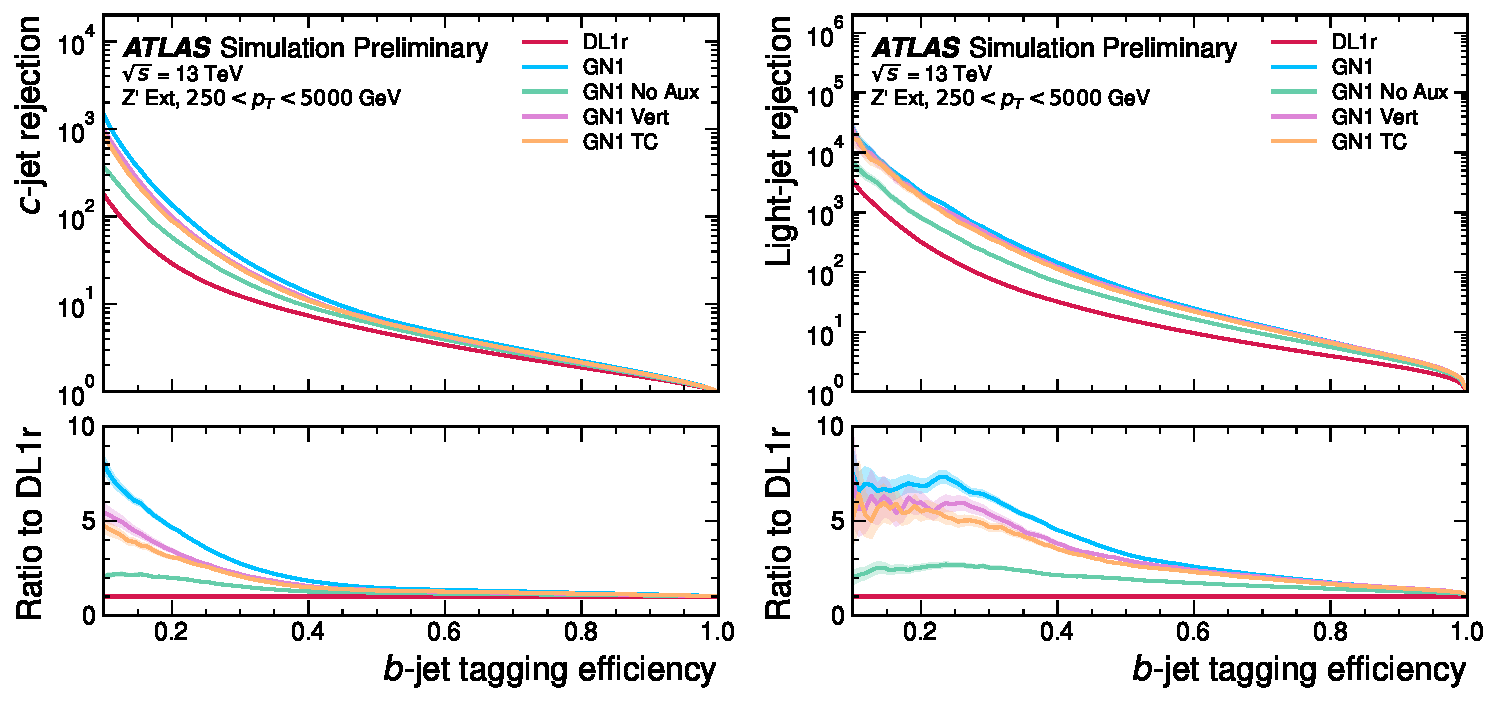
\includegraphics[width=\textwidth]{chapters/gnn_tagger/figs/results/ablations/zprime/zprime_roc_btag.pdf}
    \caption{The \cjet (left) and \ljet (right) rejections as a function of the \bjet tagging efficiency for \Zprime jets with \Zprimept, for the nominal \GNN, in addition to configurations where no (\GNN No Aux), only the track classification (\GNN TC) or only the vertexing (\GNN Vert) auxiliary objectives are deployed \cite{ATL-PHYS-PUB-2022-027}. The ratio to the performance of the \DLr algorithm is shown in the bottom panels. A value of $\fc = 0.018$ is used in the calculation of \Db for \DLr and $\fc = 0.05$ is used for \GNN.}
    \label{fig:zprime_btag_roc_ab}
\end{figure}


\subsection{Inclusion of Low-Level Vertexing Algorithms}\label{sec:gnn_low_level_vert_impact}

As already mentioned, \GNN does not include any inputs from the low-level tagging algorithms, including the vertexing algorithms SV1 and JetFitter \cite{FTAG-2018-01}.
Since these algorithms are known to play a key role in contributing to the performance of \DLr, it was necessary to study whether their inclusion in \GNN resulted in further performance improvements.
In a dedicated training of \GNN the SV1 and JetFitter tagger outputs were added to the \GNN jet classification network as an input, similar to how they are used in \DLr.
These outputs include information on the reconstructed vertices, including the number of vertices, and the properties of the highest ranking reconstructed vertex (in the case of JetFitter)\todo{determine ranking}.
In addition, the index of the reconstructed SV1 or JetFitter vertices were included as two track-level inputs to \GNN.
These indices were also used to construct an an input feature for the edge classification network used to identify vertices, which was given a value of one if the track-pair were from a common reconstructed SV1 or JetFitter vertex, and zero otherwise.
The jet classification performance of this \GNN model was not significantly different to the baseline model, and in some cases the performance was slightly reduced.
\GNN does not benefit from the inclusion of information from SV1 and JetFitter, indicating that the model is able to reconstruct the relevant information provided by these low-level algorithms.
The study also demonstrates that the model can function as a highly performant standalone tagger that does not require (beyond retraining) any manual optimisation to achieve good performance in a wide range of phase spaces.
A dedicated look at the vertexing performance of \GNN with some comparisons to SV1 and JetFitter is found in \cref{sec:gnn_vert_perf}




\subsection{Jet Display Diagrams}

The auxiliary training objectives of \GNN allow for improved model interpretability, which is especially important for a monolithic approach as the low level taggers, which provide useful physical insight, are no longer present.
\cref{fig:bjet_diag_1,fig:bjet_diag_2} provide example comparisons of the true origin and vertexing information compared with the predicted values from \GNN, SV1 and JetFitter.
Such comparisons can be used to provide an indication that \GNN reconstructs the correct representation of the jet structure, and may also help to identify limitations of the model.
In the figures, the tracks in the jet are indexed twice on each of the $x$- and $y$-axes, and tracks are  grouped into vertices along with other tracks as indicated by common markings in the relevant rows and columns.

In \cref{fig:bjet_diag_1}, \GNN correctly groups the three primary tracks as having come from the primary vertex.
The \bhadron and $b\rightarrow c$-hadron decay vertices are also correctly predicted, and the origin of the tracks in each is correct.
There is a single OtherSecondary track which \GNN incorrectly predicts as having come pileup.
Meanwhile SV1 (by design) merges the two heavy flavour decay vertices, but incorrectly includes a track from the primnary vertex.
JetFitter reconstructs two vertices, one which is a combination of two tracks from different truth vertices and two other single track vertices in each of the heavy flavour vertices.
\GNN also predicts the flavour of the jet with a high degree of certainty.

Similarly, \cref{fig:bjet_diag_1} shows that \GNN is able to relatively accurately predict the origin and vertex information of tracks inside a jet.
The pileup tracks and primary vertex tracks are correctly identified, and the heavy flavour decay tracks are also correctly identified with the exception of one of the \bhadron decay tracks.
Again, SV1 merges the two heavy flavour decay vertices along with a track from pileup, while JetFitter shows signs of being underconstrained by reconstructing two single track vertices, one with a pileup track and one with a track from a $b\rightarrow c$-hadron decay.

\begin{figure}[!p]
    \centering
    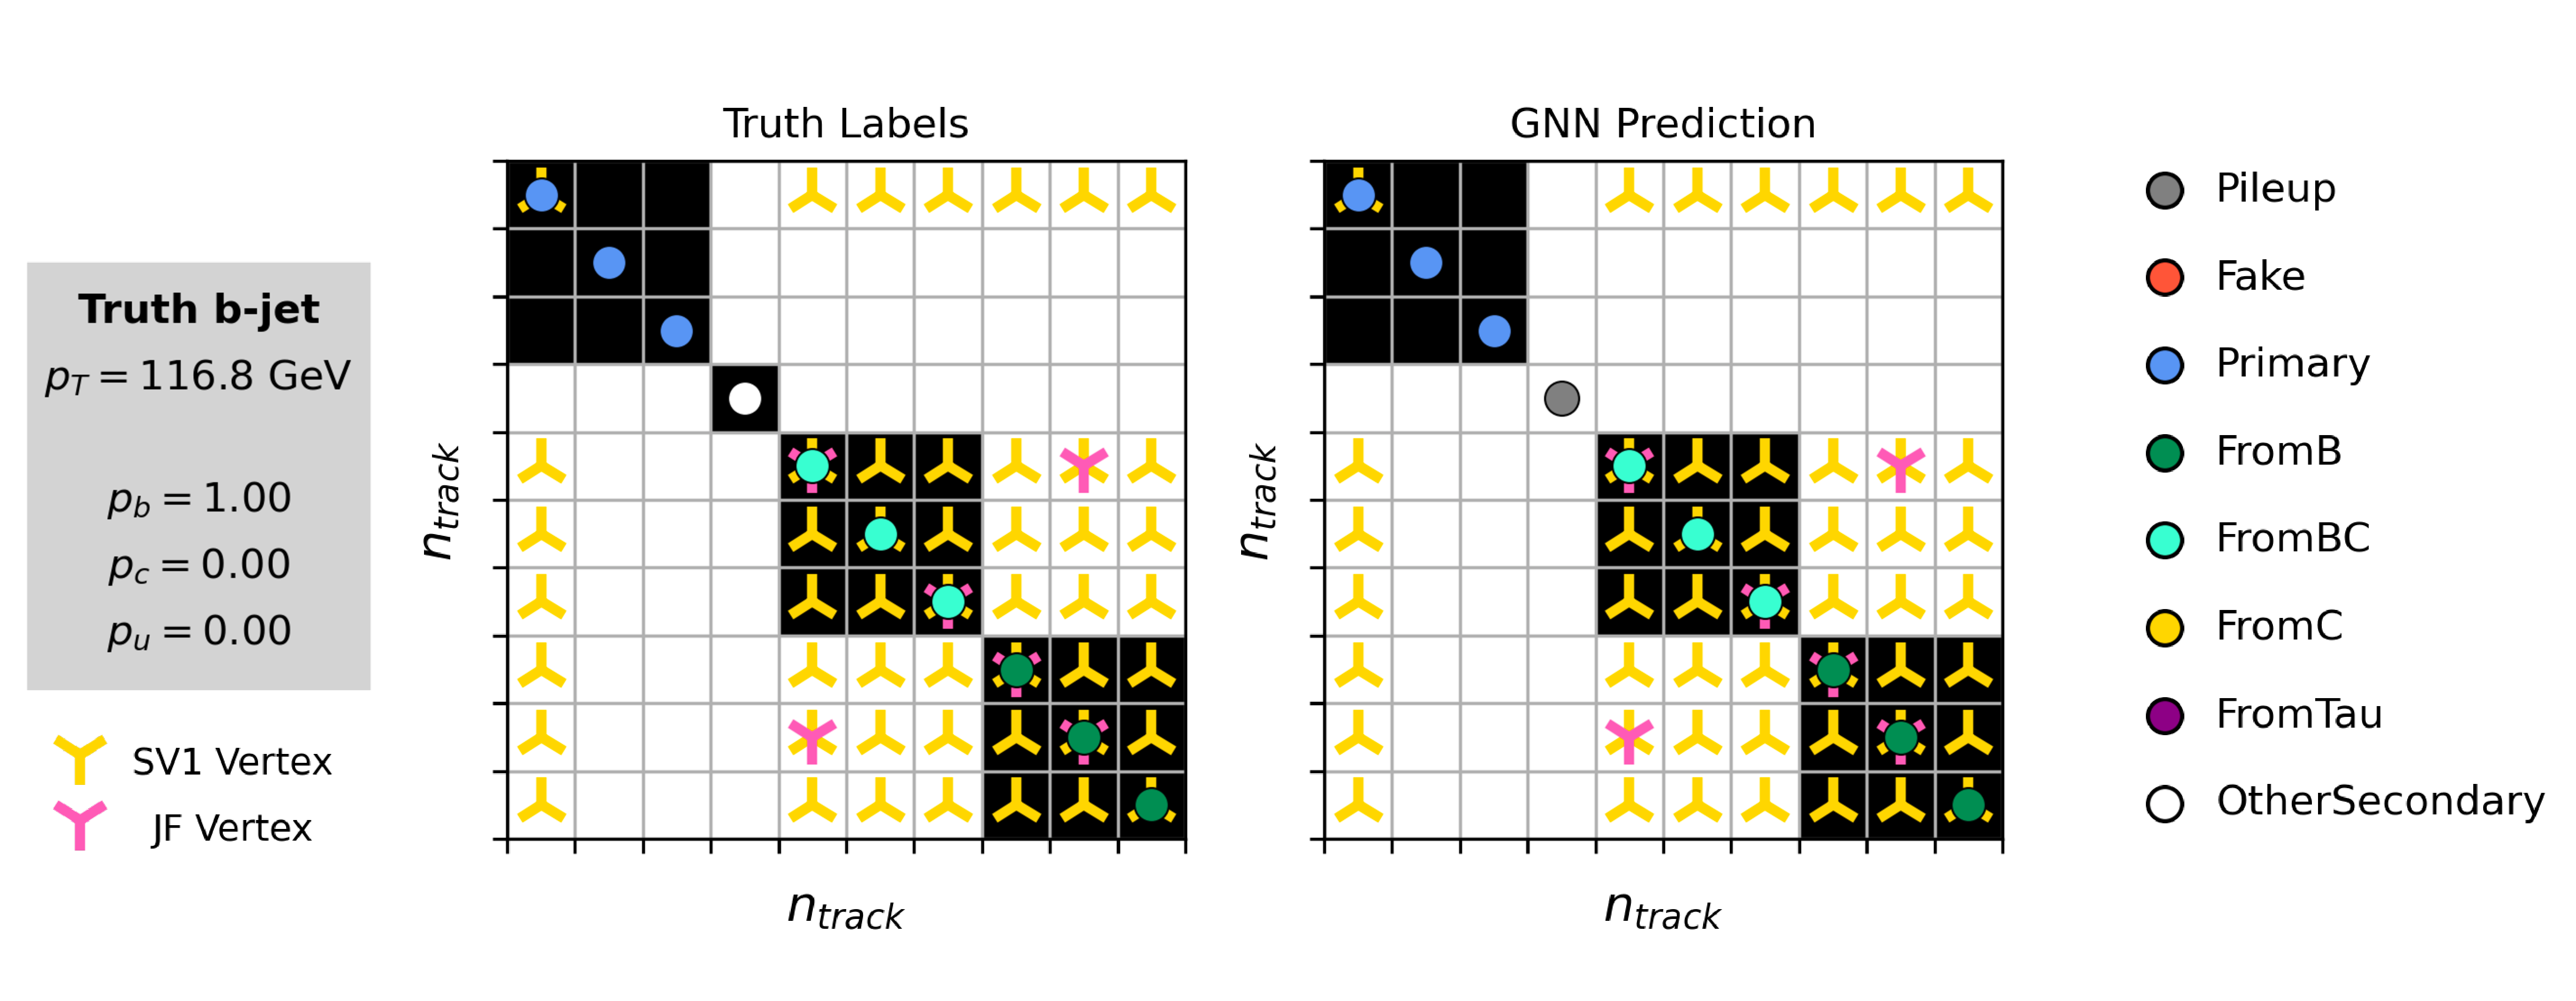
\includegraphics[width=0.95\textwidth]{chapters/gnn_tagger/figs/bjet_vertex.pdf}
    \caption{
        A schematic showing the truth track origin and vertex information (left) compared with the predictions from \GNN (right).
        The diagrams show the truth (left) and predicted (right) structure of a \bjet.
        The shaded black boxes show the groupings of tracks into different vertices.
        Vertices reconstructed by SV1 and JetFitter are also marked.
        Class probabilities $p_b$, $p_c$ and $p_u$ are rounded to three significant figures.
        \GNN improves over SV1 and JetFitter by successfully determining the origins and vertex compatability of all the tracks in the jet with the exception of the truth OtherSecondary track, which is misidentified as pileup.
    }
    \label{fig:bjet_diag_1}
 \end{figure}

 \begin{figure}[!p]
    \centering
    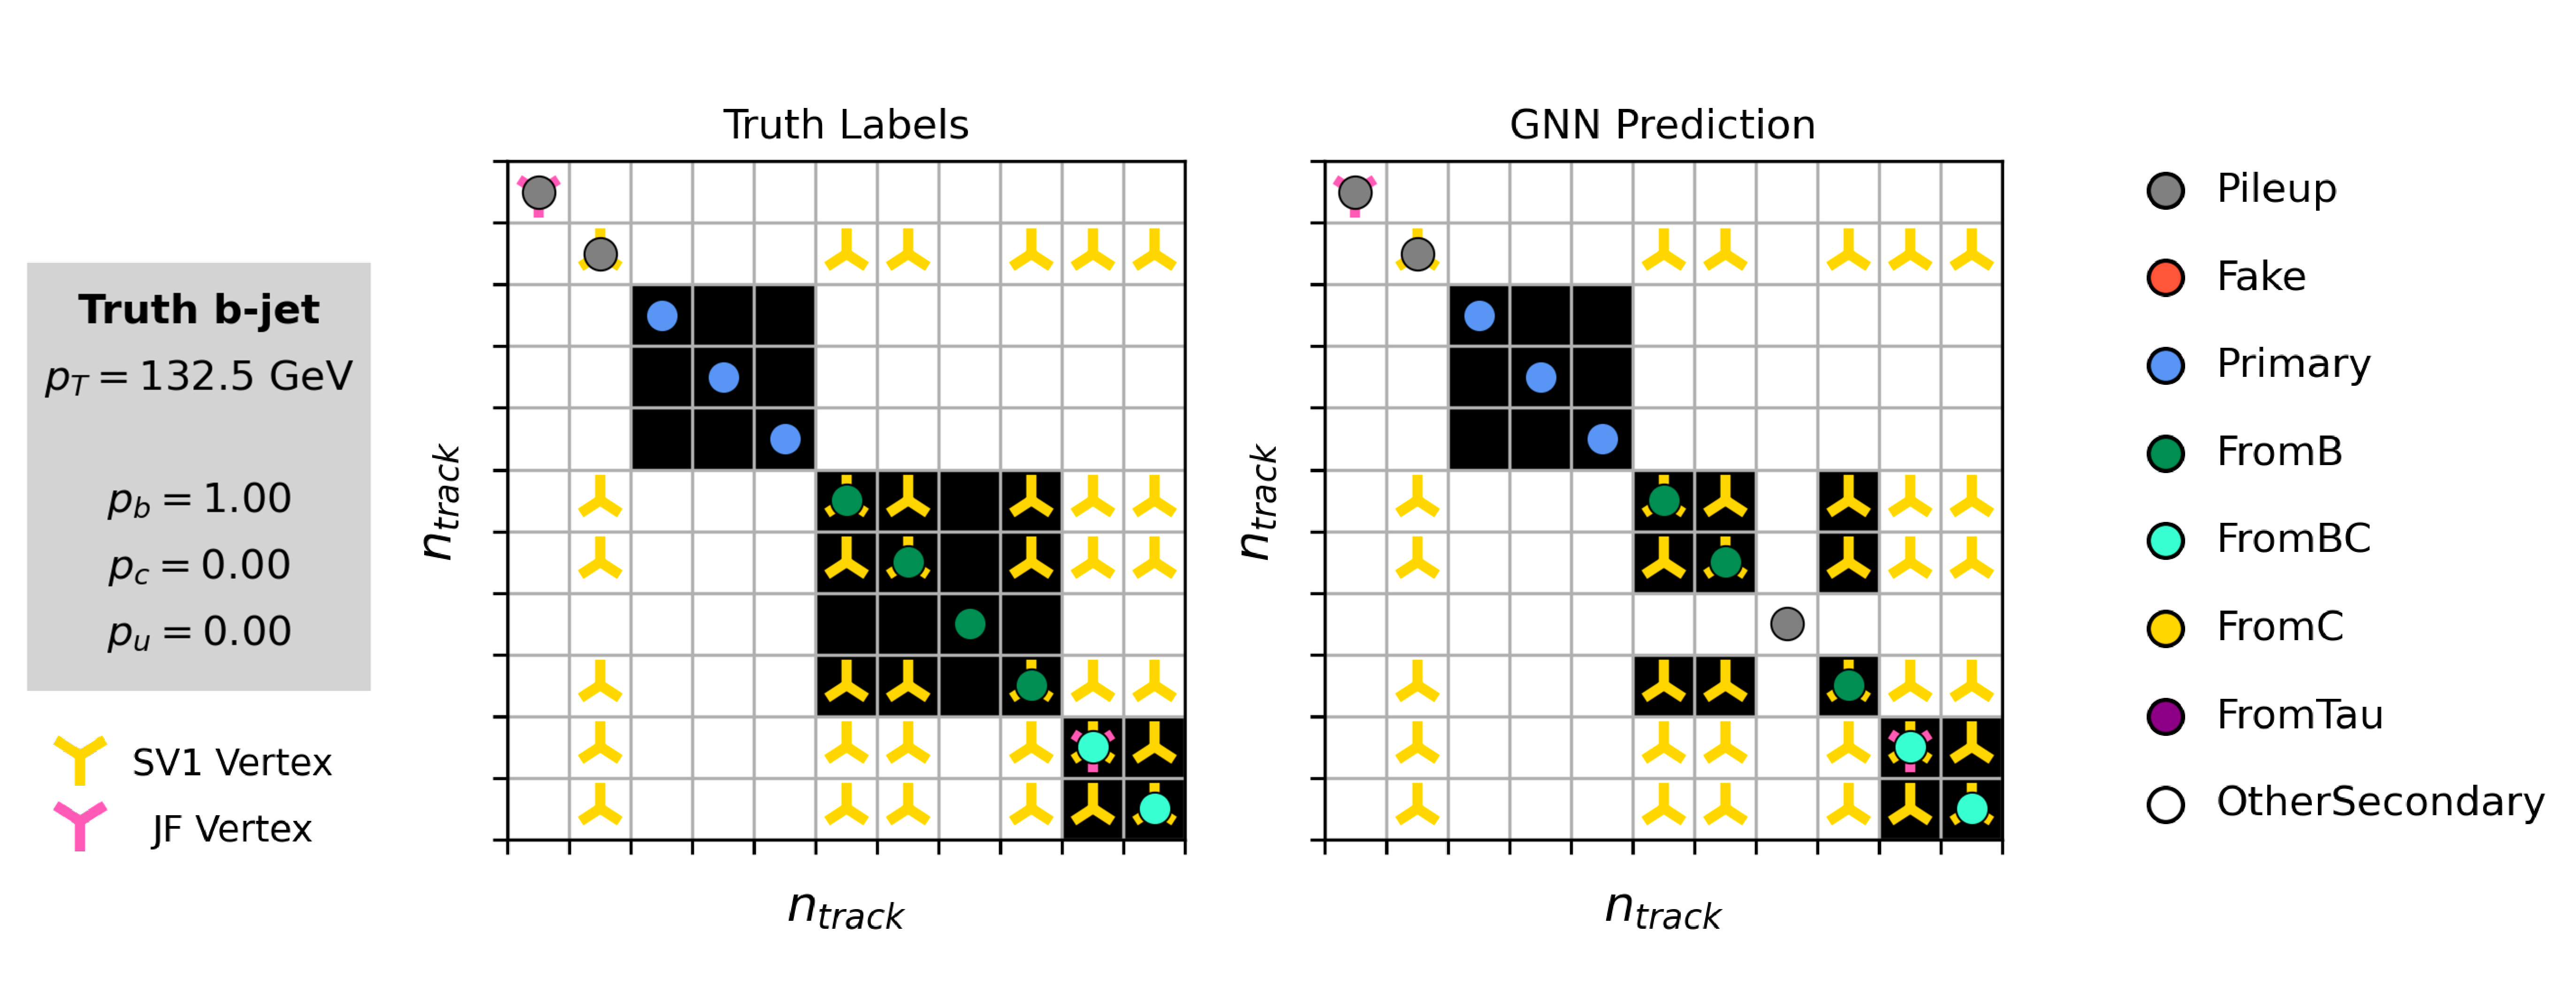
\includegraphics[width=0.95\textwidth]{chapters/gnn_tagger/figs/bjet_vertex2.pdf}
    \caption{
        A schematic showing the truth track origin and vertex information (left) compared with the predictions from \GNN (right).
        The diagrams show the truth (left) and predicted (right) structure of a \bjet.
        The shaded black boxes show the groupings of tracks into different vertices.
        Vertices reconstructed by SV1 and JetFitter are also marked.
        Class probabilities $p_b$, $p_c$ and $p_u$ are rounded to three significant figures.
        \GNN improves over SV1 and JetFitter by successfully determining the origins and vertex compatability of all but one tracks in the jet.
    }
    \label{fig:bjet_diag_2}
 \end{figure}

 

\subsection{Vertexing Performance}\label{sec:gnn_vert_perf}

From the track-pair vertex prediction described in \cref{sec:aux-train-objectives}, tracks can be partitioned into compatible groups representing vertices (see \cite{serviansky2020set2graph}).
As such, \GNN can perform vertex ``finding'', but not vertex ``fitting'', i.e. the reconstruction of a vertex's properties, which currently still requires the use of a dedicated vertex fitter.
In order to study the performance of the different vertexing tools, the truth vertex label of the tracks, discussed in \cref{sec:aux-train-objectives}, are used.
To estimate the efficiency with which \GNN manages to find vertices inclusively, vertices containing tracks identified as coming from a \bhadron are merged together and compared to the inclusive truth decay vertices that result from a \bhadron decay (where if there are multiple distinct truth vertices from a \bhadron decay they are also merged together).
Vertices are compared with the target truth vertex and the number of correctly and incorrectly assigned tracks is computed.
Since secondary vertex information is only recovered for reconstructed tracks, a vertex finding efficiency of $100\%$ denotes that all possible secondary vertices are found given the limits set by the track reconstruction efficiency.
A vertex is considered matched if it contains at least $65\%$ of the tracks in the corresponding truth vertex, and has a purity of at least $50\%$.
\GNN manages to achieve an inclusive reconstruction efficiency in \bjets of $\sim80\%$, demonstrating that it effectively manages to identify the displaced vertices from \bhadron decays.


%In order to study the performance of the different vertexing tools inside \bjets, the truth vertex label of the tracks, discussed in \cref{sec:aux-train-objectives}, is used.
%The reconstructed vertices from \GNN, SV1 and JetFitter are compared to the target truth vertices in order to calculate the efficiencies of the different vertexing tools.
%Since secondary vertex information is only recovered for reconstructed tracks, an efficiency of $100\%$ here denotes that all possible secondary vertices are recovered given the limited track reconstruction efficiency.

There are several caveats to a comparison of the vertexing tools which are a result of the different approaches they take to vertexing.
SV1 and JetFitter are designed to only find secondary vertices in the jet, whereas \GNN is also trained to determine which tracks in the jet belong to the primary vertex (the vertex of the hard scatter $pp$ interaction).
To account for this the \GNN vertex with the largest number of predicted primary tracks is excluded from the vertex finding efficiency calculation.
While JetFitter and \GNN aim to resolve each displaced vertex inside the jet, such that secondary vertices from \bhadron decays are found separately to tertiary vertices from $b \rightarrow c$ decay chains, SV1 by design attempts to find a single inclusive vertex per jet.
This inclusive vertex groups tracks from the \bhadron decay itself (FromB) and tracks from $b \rightarrow c$ decays (FromBC).
In order to fairly compare the performance of the different tools, both the exclusive and inclusive vertex finding efficiency is studied.
For the exclusive vertex finding case JetFitter and \GNN can be directly compared, while a comparison with SV1 is not possible due to the aforementioned design constraints.
The inclusive vertex finding performance of all three tools can be compared using the procedure outlined below.

The starting point for the secondary vertex finding efficiency in both the exclusive and inclusive cases is to select truth secondary vertices, defined as those containing only inclusive \bhadron decays.
For exclusive vertex finding, these truth secondary vertices can be used directly as the demoninator for the efficiency calculation.
Meanwhile for the inclusive efficiency all such truth secondary vertices in the jet are merged into a single inclusive target vertex.
Correspondingly, for the inclusive vertex finding case, the vertices found by JetFitter are merged into a single vertex, and the vertices found by \GNN, which contain at least one predicted \bhadron decay track, are also merged similarly.
SV1 does not require any vertex merging.
Only jets containing a single \bhadron at truth level are considered.

Next, vertices in the jet found by the different vertexing tools are compared with the target truth vertices.
The number of correctly and incorrectly assigned tracks is computed.
In order to call a vertex efficient, it is required to contain at least $65\%$ of the tracks in the corresponding truth vertex, and to have a purity of at least $50\%$.
Single track vertices are required to have a purity of $100\%$.
Additionally, for \GNN only, at least one track in the vertex is required to have a predicted heavy flavour origin.



Vertex finding efficiencies for \ttbarbjets are displayed as a function of \pt separately for the inclusive and exclusive approaches in \cref{fig:ttbar_vert_eff}.
For \ttbarbjets with \ttbarpt, the exclusive vertex finding efficiency of JetFitter and \GNN is relatively flat as a function of \pt.
For the truth secondary vertices in this \pt region, JetFitter efficiently finds approximately \pct{40} and \GNN finds approimately \pct{55}.
When finding vertices inclusively the vertex finding efficiency is generally higher.
An increased dependence on \pt is also visible for JetFitter and SV1. As the jet \pt increases from \SI{20}{\GeV} to \SI{100}{\GeV}, the efficiency of JetFitter increases from \pct{60} to \pct{65}.
In the same range, the efficiency of SV1 increases from \pct{60} to \pct{75}.
\GNN displays less dependence on \pt than JetFitter and SV1, efficiently finding upwards of \pct{80} of vertices in \bjets in this \pt region. 
For \bjets with $\pt > \SI{100}{\GeV}$, JetFitter finds approximately \pct{65} of vertices, SV1 finds approimately \pct{75} of vertices, and \GNN finds approximately \pct{80} of vertices.

\begin{figure}[!htbp]
    \centering
    \begin{subfigure}[b]{0.48\textwidth}
        \centering
        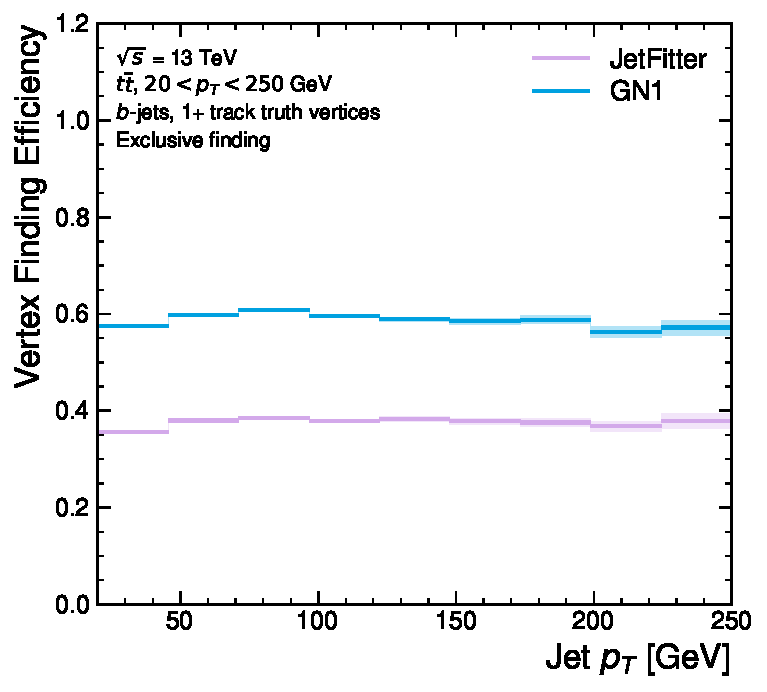
\includegraphics[width=\textwidth]{chapters/gnn_tagger/figs/results/tracks/ttbar/ttbar_bjet_vert_eff_1+_track_excl.pdf}
        %\caption{sub}
        %\label{fig:sub}
    \end{subfigure}
    \quad
    \begin{subfigure}[b]{0.48\textwidth}
        \centering
        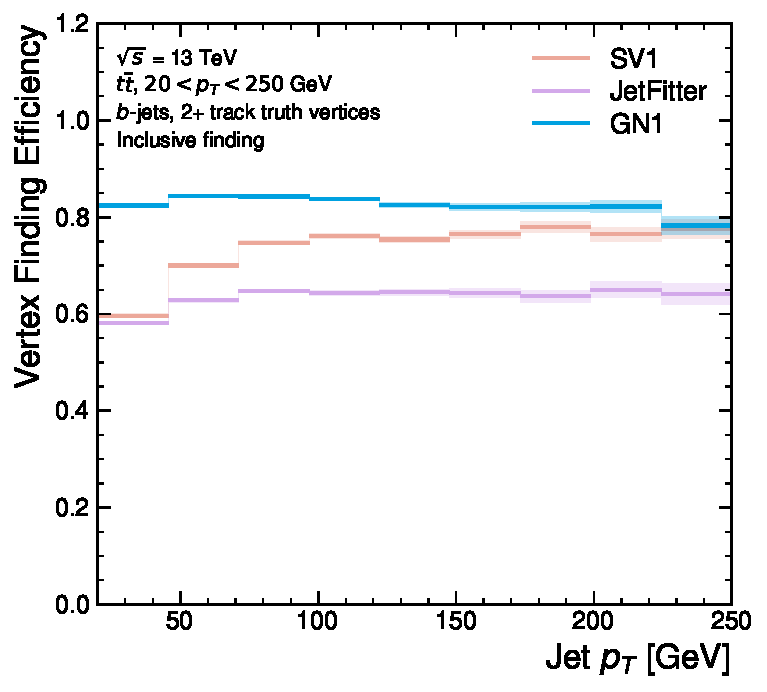
\includegraphics[width=\textwidth]{chapters/gnn_tagger/figs/results/tracks/ttbar/ttbar_bjet_vert_eff_2+_track_incl.pdf}
        %\caption{sub}
        %\label{fig:sub}
    \end{subfigure}
    \caption{
        Vertex finding efficiency as a function of jet \pt for \ttbarbjets using the exclusive (left) and inclusive (right) vertex finding approaches.
        The exclusive vertexing approach includes single track vertices while the inclusive approach requires vertices to contain at least two tracks.
        Efficient vertex finding requires the recall of at least $65\%$ of the tracks in the truth vertex, and allows no more than $50\%$ of the tacks to be included incorrectly.
        Binomial error bands are denoted by the shaded regions.}
    \label{fig:ttbar_vert_eff}
\end{figure}

\cref{fig:zprime_vert_eff} compares the exclusive vertex finding efficiencies of JetFitter and \GNN for multitrack vertices.
For \Zprimebjets, the vertex finding efficiency drops steeply with increasing \pt up until $\pt = \SI{3}{\TeV}$.
\GNN outperforms SV1 and JetFitter across the \pt spectrum.
In the first bin, the efficiency of \GNN is $75\%$, while the efficiencies of SV1 and JetFitter are around $60\%$.
The efficiency of SV1 drops rapidly to almost zero above \SI{3}{\TeV}, while JetFitter and \GNN retain approximately \pct{25} and \pct{30} efficiency respectively.
JetFitter finds $45\text{\nobreakdash-}50\%$ of vertices in \ttbarbjets, while \GNN finds $60\text{\nobreakdash-}65\%$.
For \Zprimebjets, JetFitter finds $35\%$ of vertices in the first bin, dropping to $20\%$ of vertices above \SI{2}{\TeV}.
\GNN finds $55\%$ of vertices in the first bin, dropping to $30\%$ above \SI{2}{\TeV}.

\begin{figure}[!htbp]
    \centering
    \begin{subfigure}[b]{0.48\textwidth}
        \centering
        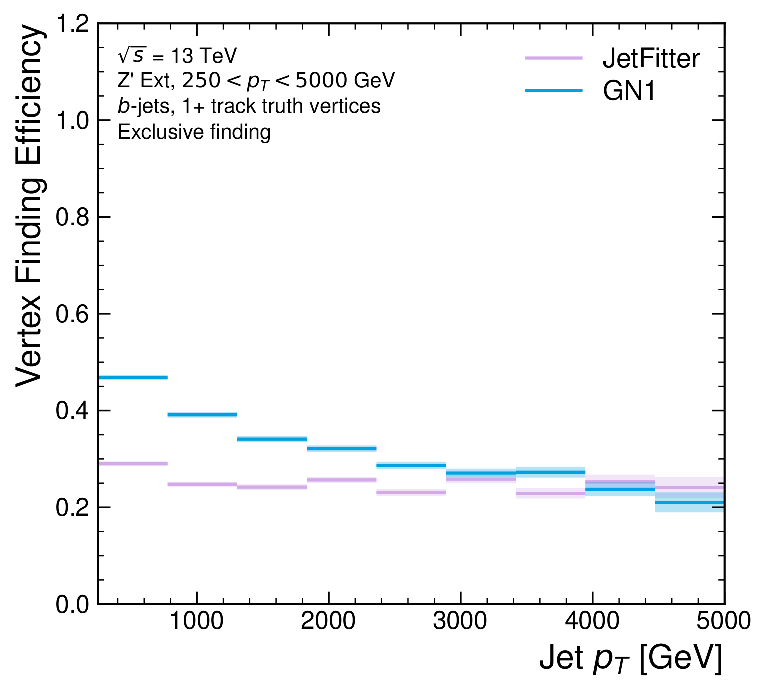
\includegraphics[width=\textwidth]{chapters/gnn_tagger/figs/results/tracks/zprime/zprime_bjet_vert_eff_1+_track_excl.pdf}
        %\caption{sub}
        %\label{fig:sub}
    \end{subfigure}
    \quad
    \begin{subfigure}[b]{0.48\textwidth}
        \centering
        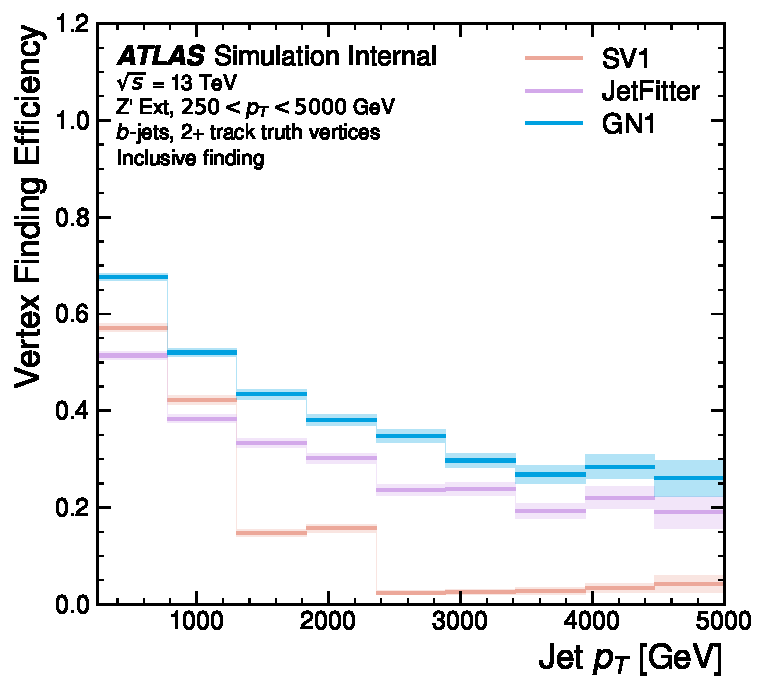
\includegraphics[width=\textwidth]{chapters/gnn_tagger/figs/results/tracks/zprime/zprime_bjet_vert_eff_2+_track_incl.pdf}
        %\caption{sub}
        %\label{fig:sub}
    \end{subfigure}
    \caption{
        Inclusive vertex finding efficiency for multitrack truth vertices in \ttbarbjets (left) and \Zprimejets (right) as a function of jet \pt.
        The exclusive vertexing approach includes single track vertices while the inclusive approach requires vertices to contain at least two tracks.
        Efficient vertex finding requires the recall of at least $65\%$ of the tracks in the truth vertex, and allows no more than $50\%$ of the tacks to be included incorrectly.
        }
    \label{fig:zprime_vert_eff}
\end{figure}


%\GNN also outperforms JetFitter in single track exclusive vertex finding as shown in \cref{fig:vert_eff_1track_excl}, except at $\pt > 3 ~\TeV$, where the efficiency of JetFitter starts to increase.
%As shown in \cref{fig:vert_eff_1track_excl}, JetFitter has a high rate to find vertices in \ljets in this region of phase space.
%\cref{fig:vert_eff_1track_excl} shows the rate at which the different tools find vertices within \ljets as a function of jet \pt. 
%Found vertices in \ljets can correspond to real displaced truth vertices caused by for example material interactions, or can be comprised of tracks which do not originate from a common displaced truth vertex (``fake'' vertices).
%The SV1 rate remains low at under $10\%$ for \ttbarZprimeljets.
%
%\begin{figure}[!htbp]
%    \centering
%    \begin{subfigure}[b]{0.48\textwidth}
%        \centering
%        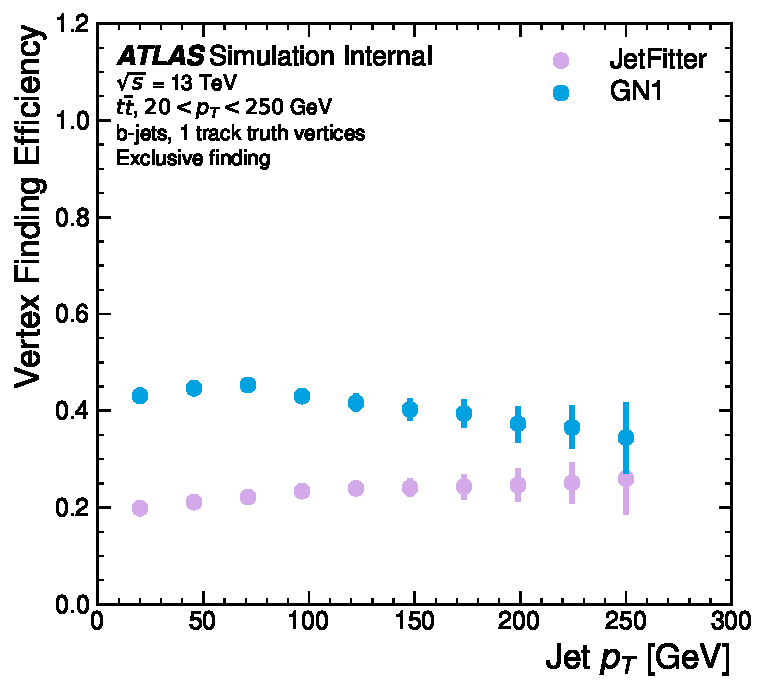
\includegraphics[width=\textwidth]{fig/results/tracks/ttbar/ttbar_vert_eff_1_track_excl.pdf}
%        %\caption{sub}
%        %\label{fig:sub}
%    \end{subfigure}
%    \quad
%    \begin{subfigure}[b]{0.48\textwidth}
%        \centering
%        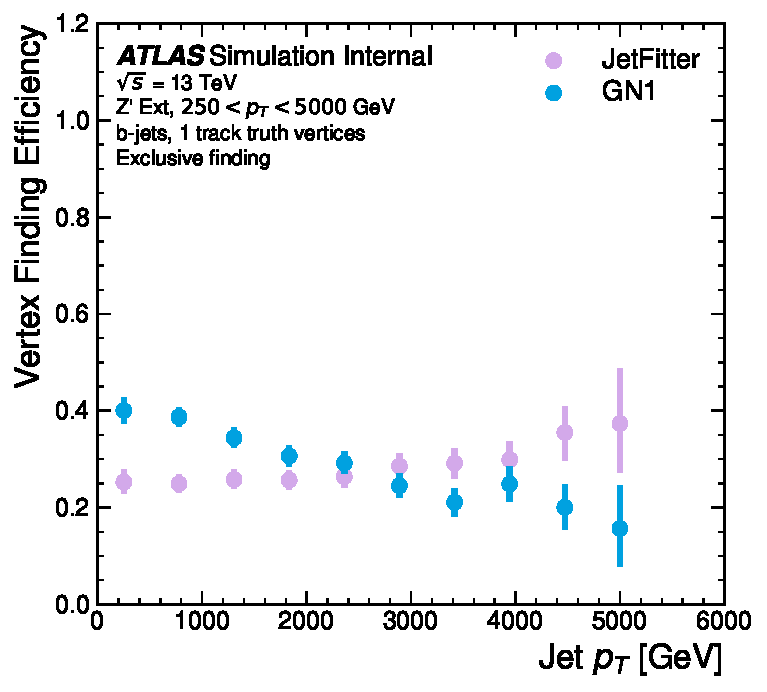
\includegraphics[width=\textwidth]{fig/results/tracks/zprime/zprime_vert_eff_1_track_excl.pdf}
%        %\caption{sub}
%        %\label{fig:sub}
%    \end{subfigure}
%    \caption{Exclusive vertex finding efficiency for single track truth vertices in \ttbarbjets (left) and \Zprimejets (right) as a function of jet \pt. Efficient vertex finding in single track vertices requires the truth and found vertex to match exactly.}
%    \label{fig:vert_eff_1track_excl}
%\end{figure}
%
%For \ttbarljets, the rate of found JetFitter (\GNN) vertices increases as a function of \pt from 0.3 to 0.7 (0.5 to 1.1) vertices per jet.
%For \Zprimeljets, the vertexing rate of JetFitter plateaus above $3 ~\TeV$ at 2 vertices per jet, while the \GNN rate decreases steadily from 1.4 vertices for $\pt < 1 ~\TeV$ to 0.8 vertices above $4 ~\TeV$.
%By requiring that vertices found by \GNN also include at least one track with a predicted heavy flavour origin, as was done for the vertexing efficiency, the rate of \GNN vertices in \ljets can be suppressed to levels similar as found by SV1.
%Overall these results indicate that the \GNN model is able to efficiency find vertices when compared with SV1 and JetFitter.
%
%\begin{figure}[!htbp]
%    \centering
%    \begin{subfigure}[b]{0.48\textwidth}
%        \centering
%        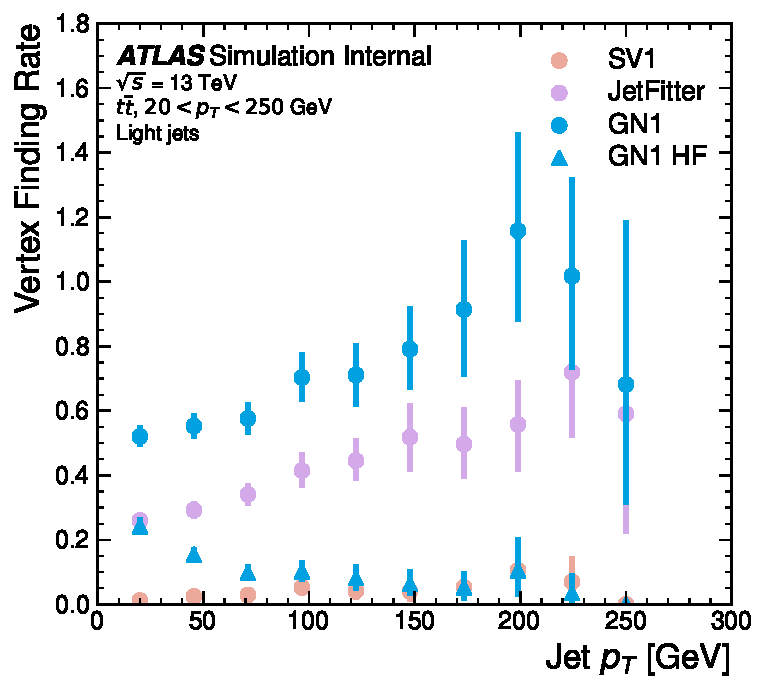
\includegraphics[width=\textwidth]{fig/results/tracks/ttbar/ttbar_vert_fake_all_v2.pdf}
%        %\caption{sub}
%        %\label{fig:sub}
%    \end{subfigure}
%    \quad
%    \begin{subfigure}[b]{0.48\textwidth}
%        \centering
%        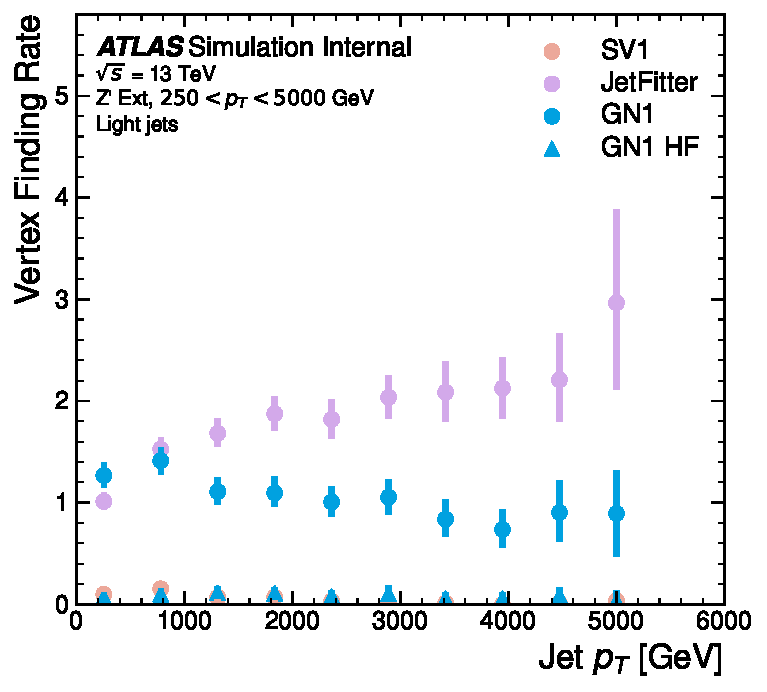
\includegraphics[width=\textwidth]{fig/results/tracks/zprime/zprime_vert_fake_all_v2.pdf}
%        %\caption{sub}
%        %\label{fig:sub}
%    \end{subfigure}
%    \caption{Vertex finding rate in \ljets for truth vertices in \ttbarbjets (left) and \Zprimejets (right) as a function of jet \pt. Found vertices in \ljets can correspond to real displaced vertices from secondary interactions or can be fake vertices. \GNN has a relatively high rate to find vertices in \ljets, though this can be suppressed by requiring that at least one track in the vertex have a predicted heavy flavour origin.}
%    \label{fig:vert_fake_all}
%\end{figure}



\subsection{Track Classification Performance}\label{sec:gnn_tc_perf}

One of the two auxiliary training objectives used by \GNN is to predict the truth origin of each track associated to the jet, as discussed in \cref{sec:aux-train-objectives}.
Since the equivalent information is not provided by any of the existing flavour tagging tools, a benchmark model used to predict the truth origin of each track is trained based on a standard multi-class feed-forward classification network.
The benchmark model is trained on the same tracks used for the baseline \GNN training.
The model uses precisely the same concatenated track-and-jet inputs as used by \GNN (see \cref{sec:model-inputs}), but processes only a single track at a time, meaning it cannot take into account the correlations between tracks when determining the track origin.
The model is made up of five densely connected linear layers with 200 neurons in each layer.
The performance of the model was found to be unsensitive to changes in the network structure. 

To measure the track classification performance, the area under the curve (AUC) of the receiver operating characteristic (ROC) curve is computed for each origin class, using a one-versus-all classification approach.
The AUCs for the different truth origins are averaged using both an unweighted and a weighted mean.
The unweighted mean treats the performance of each class equally, while the weighted mean uses as a weight the relative abundance of tracks of each class.
\cref{tab:track_classification_metrics} demonstrates clearly that \GNN outperforms the MLP both at \ttbarpt for \ttbarjets and at \Zprimept for \Zprimejets.
For example, \GNN can reject \pct{65} of fake tracks in \ttbarjets, while retaining more than \pct{99} of good tracks (i.e.those tracks which are not fake).
The \GNN model has two advantages over the MLP which can explain the performance improvement.
Firstly, the graph neural network architecture enables the sharing of information between tracks as discussed in \cref{sec:Architecture}.
This is likely to be beneficial since the origins of different tracks within a jet are correlated.
Secondly, the jet classification and vertexing objectives may be complementary to the track classification objective, and so the track classification performance is improved by the combined training of complementary objectives.

\begin{table}[!htbp]
  \footnotesize\centering
  \setlength{\tabcolsep}{0.5em} % for the horizontal padding
  \begin{tabular}{cc cc cc cc cc}
      \toprule\hline 
      \multicolumn{1}{l}{}    & \multicolumn{1}{l}{} & \multicolumn{2}{c}{AUC}                                 & \multicolumn{2}{c}{Precision}                           & \multicolumn{2}{c}{Recall}                              & \multicolumn{2}{c}{F1}                                  \\
      \multicolumn{1}{l}{}    & \multicolumn{1}{l}{} & \multicolumn{1}{c}{Mean} & \multicolumn{1}{c}{Weighted} & \multicolumn{1}{c}{Mean} & \multicolumn{1}{c}{Weighted} & \multicolumn{1}{c}{Mean} & \multicolumn{1}{c}{Weighted} & \multicolumn{1}{c}{Mean} & \multicolumn{1}{c}{Weighted} \\
      \cmidrule(lr){3-4} \cmidrule(lr){5-6} \cmidrule(lr){7-8} \cmidrule(lr){9-10}

      \multirow{2}{*}{\ttbar} & 
      MLP & 0.87 & 0.89 & 0.39 & 0.71 & 0.51 & 0.56 & 0.36 & 0.62 \\ & 
      GN1 & \textbf{0.92} & \textbf{0.95} & \textbf{0.51} & \textbf{0.82} & \textbf{0.64} & \textbf{0.70} & \textbf{0.51} & \textbf{0.74} 
      \\
      \multirow{2}{*}{\Zprime} & 
      MLP & 0.90 & 0.94 & 0.36 & 0.84 & 0.47 & 0.72 & 0.31 & 0.76 \\ &
      GN1 & \textbf{0.94} & \textbf{0.96} & \textbf{0.48} & \textbf{0.88} & \textbf{0.60} & \textbf{0.79} & \textbf{0.48} & \textbf{0.82} \\             
      \hline\bottomrule
  \end{tabular}
  \caption{
    The area under the ROC curves (AUC) for the track classification from \GNN, compared to a standard multilayer perceptron (MLP) trained on a per-track basis. 
    The unweighted mean AUC over the origin classes and weighted mean AUC (using as a weight the fraction of tracks from the given origin) is provided.
    \GNN, which uses an architecture that allows track origins to be classified in a conditional manner as discussed in \cref{sec:Architecture}, outperforms the MLP model for both \ttbar and \Zprime jets.
  }
  \label{tab:track_classification_metrics}
\end{table}


\cref{fig:track_origin_roc} shows the track origin classification ROC curves for the different track origins for \ttbarZprimejets.
In order to improve visual readability of the plot, the curves for the heavy flavour truth origins (FromB, FromBC and FromC) have been combined (weighted by their relative abundance), as have the Primary and OtherSecondary origins.
In \ttbarZprimejets, the AUC of all the different origin groups exceeds $0.9$, representing strong overall classification performance.
In both samples fake tracks are the easiest to classify, followed by pileup tracks.
The FromC tracks which are \chadron decay products, are the hardest to classify, possibly due to their similarity to both fragmentation tracks and \bhadron decay tracks, depending on the \chadron species in question.

\begin{figure}[!htbp]
    \centering
    \begin{subfigure}[b]{0.48\textwidth}
        \centering
        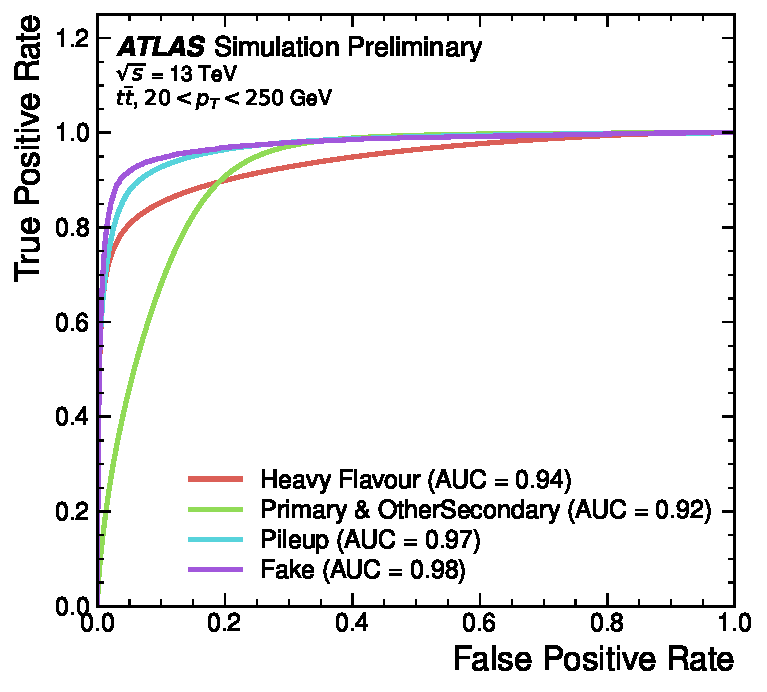
\includegraphics[width=\textwidth]{chapters/gnn_tagger/figs/results/tracks/ttbar/ttbar_origin_roc_GNNv11.pdf}
        %\caption{sub}
        %\label{fig:sub}
    \end{subfigure}
    \quad
    \begin{subfigure}[b]{0.48\textwidth}
        \centering
        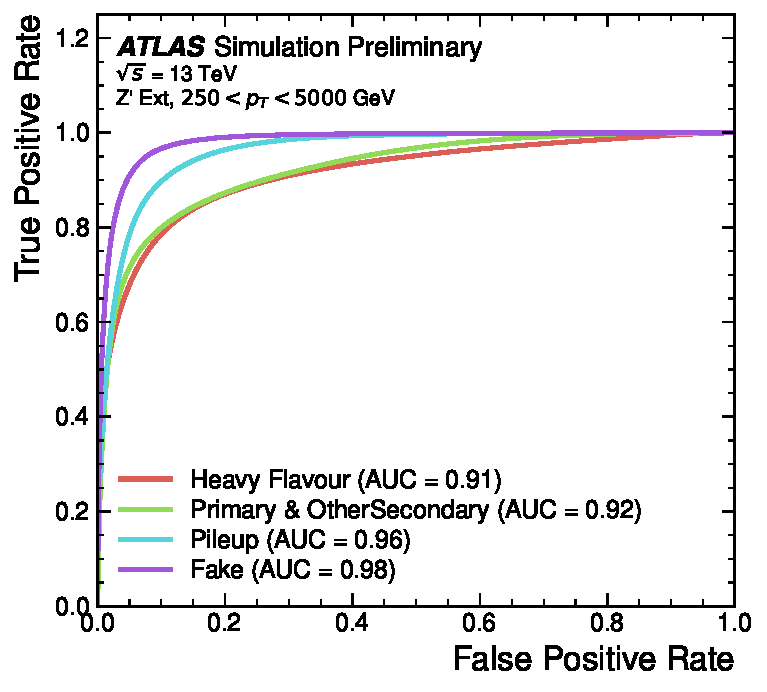
\includegraphics[width=\textwidth]{chapters/gnn_tagger/figs/results/tracks/zprime/zprime_origin_roc_GNNv11.pdf}
        %\caption{sub}
        %\label{fig:sub}
    \end{subfigure}
    \caption{
        ROC curves for the different groups of truth origin labels defined in \cref{tab:truth_origins} for \ttbarjets (left) and \Zprimejets (right) \cite{ATL-PHYS-PUB-2022-027}.
        The FromB, FromBC and FromC labels have been combined, weighted by their relative abundance, into the Heavy Flavour category, and the Primary and OtherSecondary labels have similarly been combined into a single category.
        The mean weighted area under the ROC curves (AUC) is similar for both samples.}
    \label{fig:track_origin_roc}
\end{figure}



\subsection{Looser Track Selection}\label{sec:looser_track_selection}

The track selections used to produce the main results are listed in \cref{tab:fake_track_mva_selections}.
This selection includes a cut on the number of shared silicon modules used to reconstruct the track $N^{\textnormal{Si}}_{\textnormal{shared}}$.
This value is calculated as 
%
\begin{equation}
    N^{\textnormal{Si}}_{\textnormal{shared}} = 
    \frac{N^{\textnormal{Pix}}_{\textnormal{shared}} + N^{\textnormal{SCT}}_{\textnormal{shared}}}{2}
\end{equation}
%
where $N^{\textnormal{Pix}}_{\textnormal{shared}}$ is the number of shared pixel hits and $N^{\textnormal{SCT}}_{\textnormal{shared}}$ is the number of shared SCT modules on a track.
The nominal cut used elsewhere in this thesis is $N^{\textnormal{Si}}_{\textnormal{shared}} < 2$.
As the rate of shared hits is significantly higher for \bhadron decay tracks than for other tracks, especially at \highpt, this cut rejects a significant proportion of these tracks.

\cref{fig:ttbar_gn1_loose,fig:zprime_gn1_loose} show the result of training the \GNN tagger with the full relaxation of this cut, i.e. allowing tracks with any number of shared hits.
The shared hit requirements applied by the ambiguity solver as part of track reconstruction (see \cref{sec:track_reco}) are still applied.
In addition, the maximum allowed value of \dzero is increased from \SI{3.5}{\milli\meter} to \SI{5.0}{\milli\meter}.
The results show that optimisation of the input track selection can lead to significant improvements in performance over the default selection.
For the \ttbarjets shown in \cref{fig:ttbar_gn1_loose}, the effect of loosening the track selection is limited.
This is expected due to the lower prevalence of shared hits at highly displaced tracks at lower transverse momenta.
However for \Zprimejets as shown in \cref{fig:zprime_gn1_loose}, the \lrej improves with respect to the baseline \GNN model by \pct{30}, while the \lrej improves by \pct{70} at the \WP{50}{b}.


\begin{figure}[!p]
    \centering
    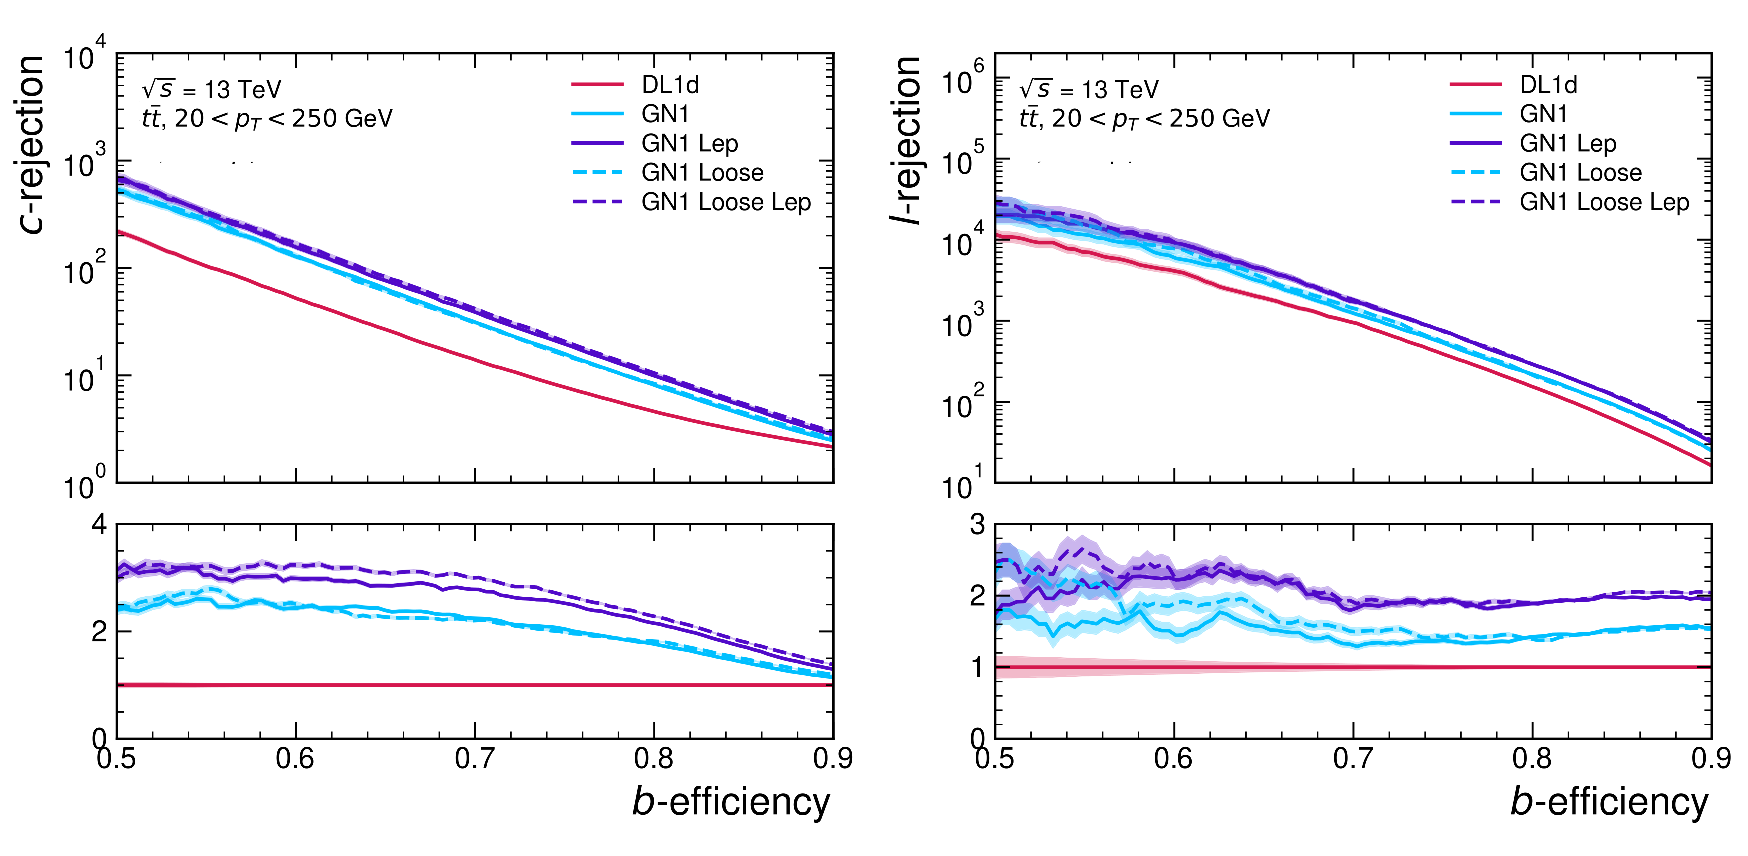
\includegraphics[width=\textwidth]{chapters/gnn_tagger/figs/gn1_loose_ttbar.pdf}
    \caption{
        The \cjet (left) and \ljet (right) rejections as a function of the \bjet tagging efficiency for \ttbar jets with \ttbarpt, for the looser track selection trainings of \GNN.
        The ratio to the performance of the DL1d algorithm \cite{ATLAS:2022qxm} is shown in the bottom panels.
        A value of $\fc = 0.018$ is used in the calculation of \Db for DL1d and $\fc = 0.05$ is used for \GNN.
        Binomial error bands are denoted by the shaded regions.
    }
    \label{fig:ttbar_gn1_loose}
\end{figure}

\begin{figure}[!p]
    \centering
    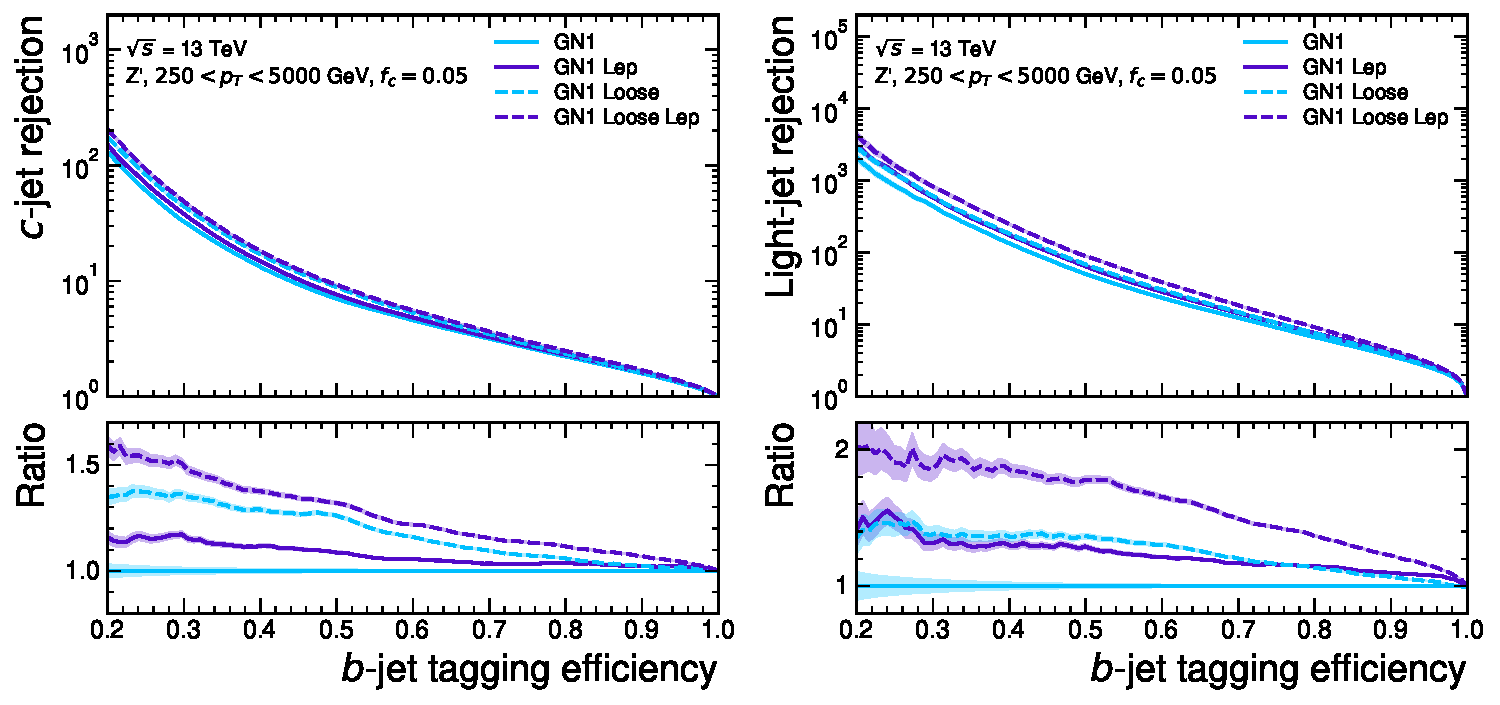
\includegraphics[width=\textwidth]{chapters/gnn_tagger/figs/gn1_loose_zprime.pdf}
    \caption{
        The \cjet (left) and \ljet (right) rejections as a function of the \bjet tagging efficiency for \Zprime jets with \Zprimept, for the looser track selection trainings of \GNN.
        The ratio to the performance of the DL1d algorithm \cite{ATLAS:2022qxm} is shown in the bottom panels.
        A value of $\fc = 0.018$ is used in the calculation of \Db for DL1d and $\fc = 0.05$ is used for \GNN.
        Binomial error bands are denoted by the shaded regions.
    }
    \label{fig:zprime_gn1_loose}
\end{figure}

Although the results demonstrate a significant performance improvement at \highpt, it is also possible that additional studies on further loosening the selection could yield further improved results.
For example the selections on the number of number of holes and the longitudinal impact parameter could be further relaxed.
The maximum number of tracks provided as input to the model could also be increased from the default value of 40.
In order to change the default tracking setup, studies investigating the modelling uncertainties of the additional tracks need to be carried out.



\section{Other Implementations of \GNN}\label{sec:gnn_trig_upgrade}

The implementation of \GNN described in this chapter has been re-used in several other contexts, demonstrating its flexibility to easily provide good jet flavour tagging performance with minimal overhead.
The model has been implemented as a \bjet tagger in the High Level Trigger (HLT) (see \cref{sec:trigger}).
The inputs to the model are the running on precision tracks and jet level quantities reconstructed after primary vertexing.
\cref{fig:gn1_trigger} shows the performance of \GNN versus a comparable DL1d model \cite{ATLAS:2022qxm}, and two versions of DIPS \cite{ATL-PHYS-PUB-2020-014}, with EMTopo and PFlow jets (see \cref{sec:jet_reco}) based on a low-precision region-of-interest based tracking pass.
The trigger implementation of \GNN improves upon the \lrej of DL1d by \pct{50} at the \WP{60}{b} for \ttbarjets with \ttbarpt.

\begin{figure}[!htbp]
    \centering
    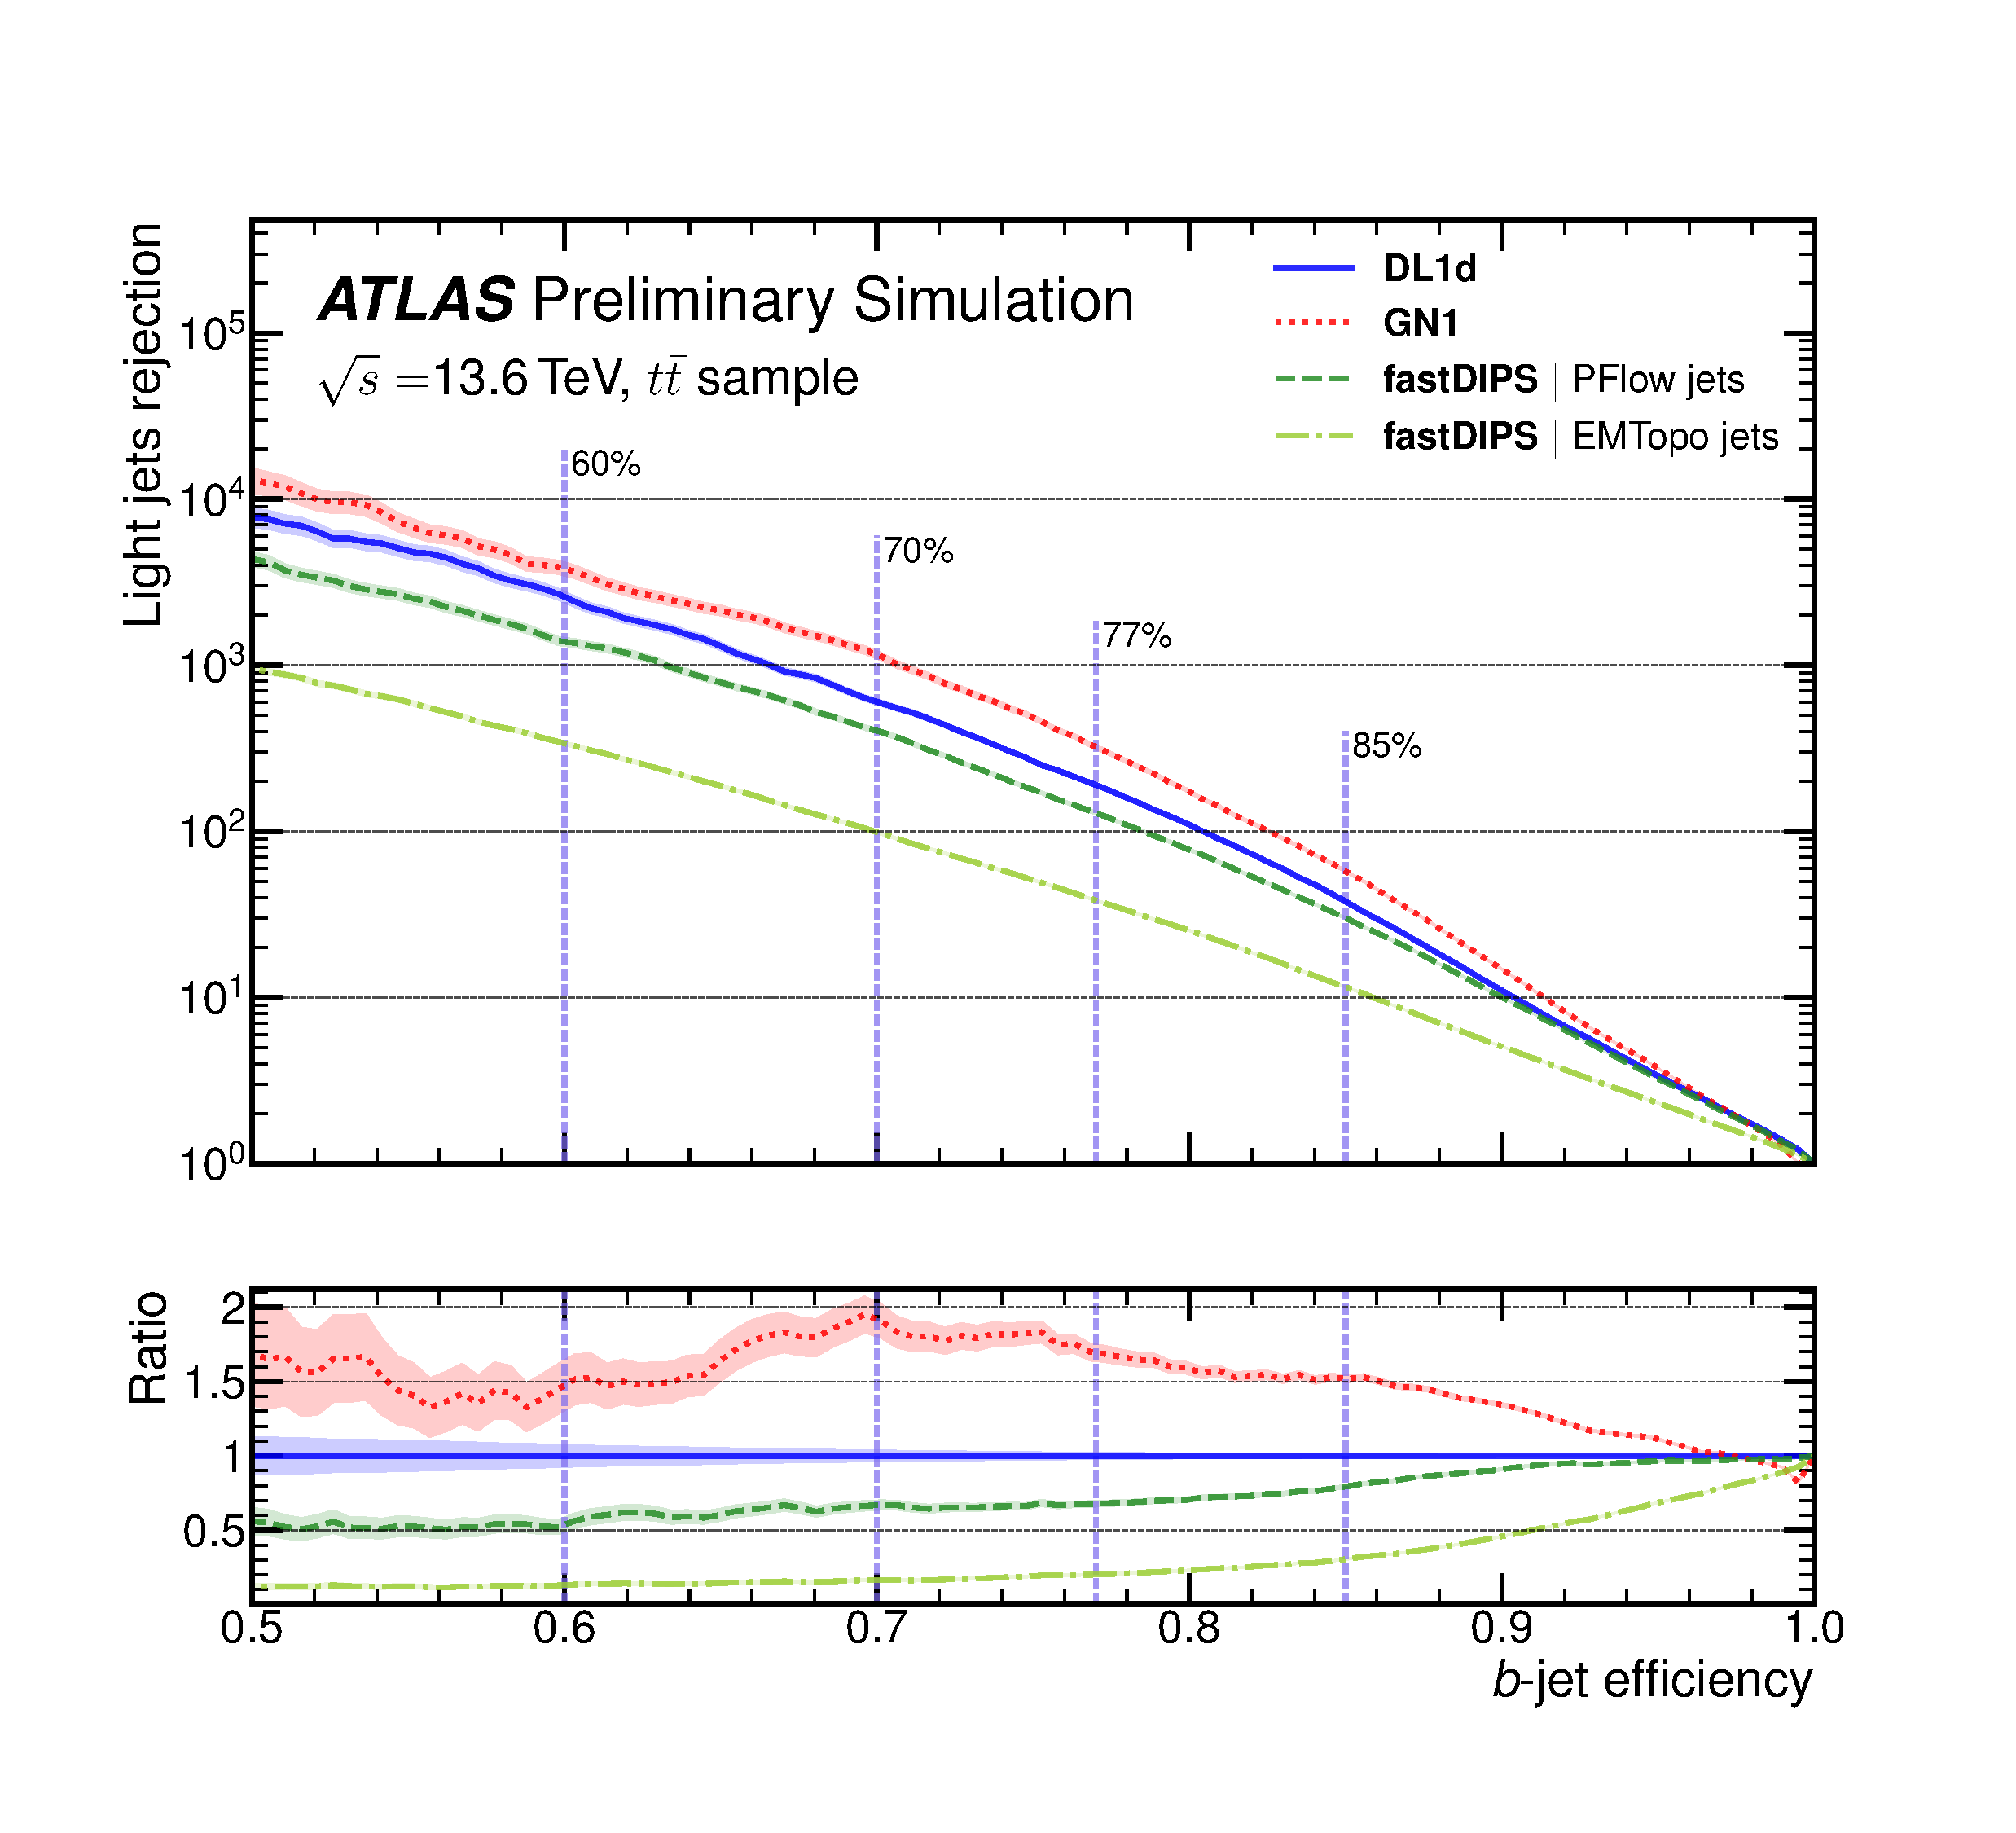
\includegraphics[width=0.6\textwidth]{chapters/gnn_tagger/figs/gn1_trigger.pdf}
    \caption{
        The \lrej as a function of the \beff \ttbarjets with \ttbarpt for events with a centre of mass energy \come{13.6} \cite{gn1-trigger}.
        The ratio to the performance of the DL1d algorithm \cite{ATLAS:2022qxm} is shown in the bottom panels.
        Binomial error bands are denoted by the shaded regions.
        The purple vertical dashed lines represent the most common working points used for b-tagging.
    }
    \label{fig:gn1_trigger}
\end{figure}


The model also demonstrates strong performance for the High Luminosity \LHC (HL-LHC), as documented in \rcite{ATL-PHYS-PUB-2022-047}.
\cref{fig:gn1_hllhc_ttbar,fig:gn1_hllhc_zprime} are reproduced from \rcite{ATL-PHYS-PUB-2022-047}.
The results show that \GNN outperforms other existing flavour tagging algorithms when trained on an entirely different detector geometry.
When compared with DL1d \cite{ATLAS:2022qxm}, \GNN improves on the \crej (\lrej) by a factor of $\sim 2$ ($\sim 2.5$) for \ttbarjets at the \WP{60}{b}.
Significant improvements in rejections are also observed for \Zprimejets.

\begin{figure}[!p]
    \centering
    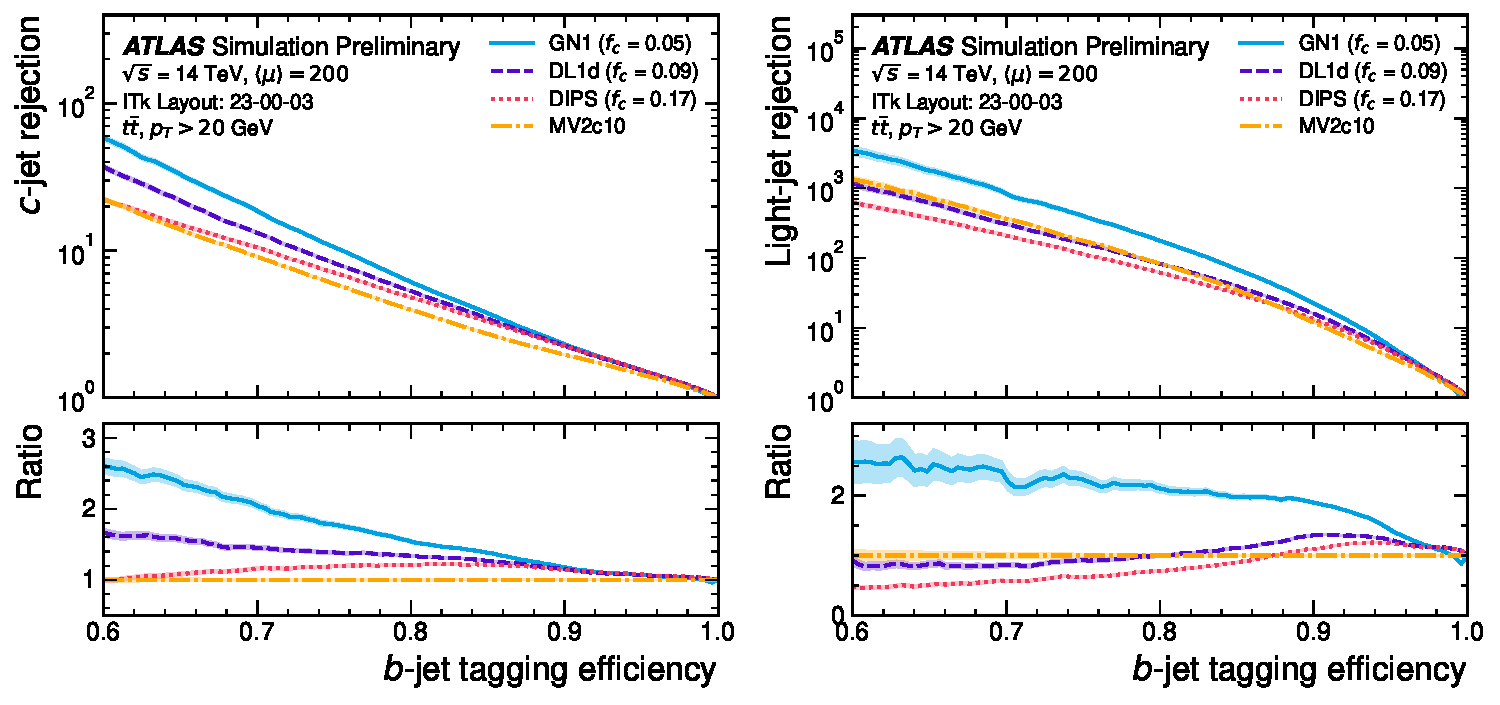
\includegraphics[width=\textwidth]{chapters/gnn_tagger/figs/gn1_hl_ttbar.pdf}
    \caption{
        The \crej (left) and \lrej (right) as a function of the \beff for \ttbarjets with \ttbarpt for events with a centre of mass energy \come{14} \cite{ATL-PHYS-PUB-2022-047}.
        The ratio to the performance of the DL1d algorithm is shown in the bottom panels.
        Binomial error bands are denoted by the shaded regions.
        The purple vertical dashed lines represent the most common working points used for b-tagging.
    }
    \label{fig:gn1_hllhc_ttbar}
\end{figure}

\begin{figure}[!p]
    \centering
    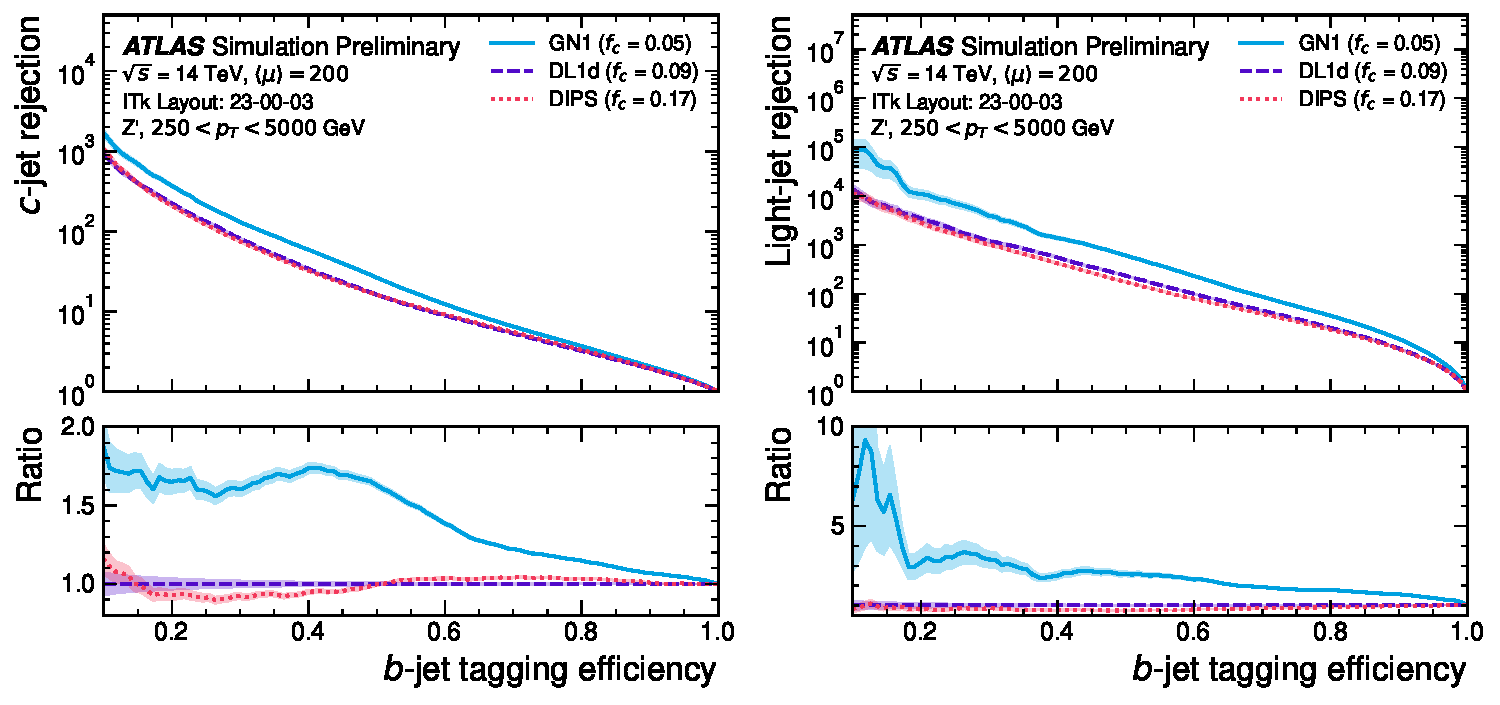
\includegraphics[width=\textwidth]{chapters/gnn_tagger/figs/gn1_hl_zprime.pdf}
    \caption{
        The \crej (left) and \lrej (right) as a function of the \beff for \Zprimejets with \Zprimept for events with a centre of mass energy \come{14} \cite{ATL-PHYS-PUB-2022-047}.
        The ratio to the performance of the DL1d algorithm is shown in the bottom panels.
        Binomial error bands are denoted by the shaded regions.
    }
    \label{fig:gn1_hllhc_zprime}
\end{figure}




%Plus trigger. There is a public trigger and the PUB Note for the upgrade studies
%I would briefly discuss both and include the references. 

%I would add one addition section before the conclusion, entitled
%‘Implementations of GN1’ or similar and show a figure from the trigger, upgrade
%and c-tagging results, to demonstrate where else it has been used so far and
%the results. Keep it short, but it would be very impactful!

\section{Conclusion}\label{sec:gnn_conclusion}

In this chapter a novel jet tagger, \GNN, is presented.
The model has a graph neural network architecture and is trained with auxiliary training objectives, which are shown to improve the performance of the basic model.
\GNN significantly improves flavour tagging performance with respect to \DLr, the current default ATLAS flavour tagging algorithm, when compared in simulated collisions.
\GNN improves \clrej for \ttbarjets with \ttbarpt by factors of \ttbclo and \ttbllo respectively at a \bjet tagging efficiency of $70\%$ when compared with \DLr.
For \Zprimejets with \Zprimept, \GNN improves the \crej by a factor of \zpbclo and \lrej by a factor of \zpbllo for a comparative \bjet efficiency of $30\%$.

Previous multivariate flavour tagging algorithms relied on inputs from low-level tagging algorithms, whereas \GNN needs no such inputs, making it more flexible. It can be easily fully optimised via a retraining for specific flavour tagging use cases, as demonstrated with \ctag and \highpt \btag, without the need for time-consuming retuning of the low-level tagging algorithms.
The model is also simpler to maintain and study due to the reduction of constituent components.

\GNN demonstrates improved track classification performance when compared with a simple per-track MLP and an efficiency of $\sim80\%$ for inclusive vertex finding in \bjets.
The model is also able to perform vertex finding, and preliminary studies suggest it outperforms previous manually optimised approaches.
The auxiliary track classification and vertex finding objectives are shown to significantly contribute to the performance in the jet classification objective, and, along with the more advanced graph neural network architecture, are directly responsible for the improvement over \DLr.

Further improvements in the $b$- and \ctagging performance are likely possible with a more thorough optimisation of the model architecture, and the integration of additional information from other parts of the \ATLAS detector.
The addition of other auxiliary training objectives, such as the truth \bhadron decay radius and transverse momentum, may also yield additional performance gains on top of the gains achieved by loosening the input track selection (demonstrated in \cref{sec:looser_track_selection}).

Additional future work includes the verification of the performance of \GNN on collision data, and the full calibration of the model so it can be used by analyses.
The flexible nature of the model means it can also be readily applied to other related problems outside of standard $b$- and \ctagging applications, as demonstrated in \cref{sec:gnn_trig_upgrade}.
Additional applications for the architecture include $X \rightarrow bb$ and $X \rightarrow cc$ tagging.
The model could also be repurposed as a pileup jet tagger, or general primary and secondary vertexing tool.

%\GNN outperforms the existing ATLAS flavour tagging algorithms as shown in \cref{sec:gnn_btag_perf,sec:gnn_ctag_perf}.
%For a \bjet efficiency of \pct{70}, the light ($c$)-jet rejection is improved by a factor of \ttbllo (\ttbclo) for jets coming from \ttbar decays with transverse momentum \ttbarpt.
%For jets coming from \Zprime decays with transverse momentum \Zprimept, the light ($c$)-jet rejection improves by a factor \zpbllo (\zpbclo) for a comparative \pct{30} \bjet efficiency.